\documentclass[twoside]{book}

% Packages required by doxygen
\usepackage{calc}
\usepackage{doxygen}
\usepackage{graphicx}
\usepackage[utf8]{inputenc}
\usepackage{makeidx}
\usepackage{multicol}
\usepackage{multirow}
\usepackage{textcomp}
\usepackage[table]{xcolor}

% Font selection
\usepackage[T1]{fontenc}
\usepackage{mathptmx}
\usepackage[scaled=.90]{helvet}
\usepackage{courier}
\usepackage{amssymb}
\usepackage{sectsty}
\renewcommand{\familydefault}{\sfdefault}
\allsectionsfont{%
  \fontseries{bc}\selectfont%
  \color{darkgray}%
}
\renewcommand{\DoxyLabelFont}{%
  \fontseries{bc}\selectfont%
  \color{darkgray}%
}

% Page & text layout
\usepackage{geometry}
\geometry{%
  letterpaper,%
  top=2.5cm,%
  bottom=2.5cm,%
  left=2.5cm,%
  right=2.5cm%
}
\tolerance=750
\hfuzz=15pt
\hbadness=750
\setlength{\emergencystretch}{15pt}
\setlength{\parindent}{0cm}
\setlength{\parskip}{0.2cm}
\makeatletter
\renewcommand{\paragraph}{%
  \@startsection{paragraph}{4}{0ex}{-1.0ex}{1.0ex}{%
    \normalfont\normalsize\bfseries\SS@parafont%
  }%
}
\renewcommand{\subparagraph}{%
  \@startsection{subparagraph}{5}{0ex}{-1.0ex}{1.0ex}{%
    \normalfont\normalsize\bfseries\SS@subparafont%
  }%
}
\makeatother

% Headers & footers
\usepackage{fancyhdr}
\pagestyle{fancyplain}
\fancyhead[LE]{\fancyplain{}{\bfseries\thepage}}
\fancyhead[CE]{\fancyplain{}{}}
\fancyhead[RE]{\fancyplain{}{\bfseries\leftmark}}
\fancyhead[LO]{\fancyplain{}{\bfseries\rightmark}}
\fancyhead[CO]{\fancyplain{}{}}
\fancyhead[RO]{\fancyplain{}{\bfseries\thepage}}
\fancyfoot[LE]{\fancyplain{}{}}
\fancyfoot[CE]{\fancyplain{}{}}
\fancyfoot[RE]{\fancyplain{}{\bfseries\scriptsize Generated on Fri Jul 31 2015 17\-:05\-:13 for A\-N\-T\-L by Doxygen }}
\fancyfoot[LO]{\fancyplain{}{\bfseries\scriptsize Generated on Fri Jul 31 2015 17\-:05\-:13 for A\-N\-T\-L by Doxygen }}
\fancyfoot[CO]{\fancyplain{}{}}
\fancyfoot[RO]{\fancyplain{}{}}
\renewcommand{\footrulewidth}{0.4pt}
\renewcommand{\chaptermark}[1]{%
  \markboth{#1}{}%
}
\renewcommand{\sectionmark}[1]{%
  \markright{\thesection\ #1}%
}

% Indices & bibliography
\usepackage{natbib}
\usepackage[titles]{tocloft}
\setcounter{tocdepth}{3}
\setcounter{secnumdepth}{5}
\makeindex

% Hyperlinks (required, but should be loaded last)
\usepackage{ifpdf}
\ifpdf
  \usepackage[pdftex,pagebackref=true]{hyperref}
\else
  \usepackage[ps2pdf,pagebackref=true]{hyperref}
\fi
\hypersetup{%
  colorlinks=true,%
  linkcolor=blue,%
  citecolor=blue,%
  unicode%
}

% Custom commands
\newcommand{\clearemptydoublepage}{%
  \newpage{\pagestyle{empty}\cleardoublepage}%
}


%===== C O N T E N T S =====

\begin{document}

% Titlepage & ToC
\hypersetup{pageanchor=false}
\pagenumbering{roman}
\begin{titlepage}
\vspace*{7cm}
\begin{center}%
{\Large A\-N\-T\-L \\[1ex]\large 0.\-0 }\\
\vspace*{1cm}
{\large Generated by Doxygen 1.8.6}\\
\vspace*{0.5cm}
{\small Fri Jul 31 2015 17:05:13}\\
\end{center}
\end{titlepage}
\clearemptydoublepage
\tableofcontents
\clearemptydoublepage
\pagenumbering{arabic}
\hypersetup{pageanchor=true}

%--- Begin generated contents ---
\chapter{Hierarchical Index}
\section{Class Hierarchy}
This inheritance list is sorted roughly, but not completely, alphabetically\-:\begin{DoxyCompactList}
\item \contentsline{section}{A\-N\-T\-L\-:\-:debug}{\pageref{dc/d7a/classANTL_1_1debug}}{}
\item \contentsline{section}{A\-N\-T\-L\-:\-:Exponentiation$<$ T $>$}{\pageref{dd/da0/classANTL_1_1Exponentiation}}{}
\begin{DoxyCompactList}
\item \contentsline{section}{A\-N\-T\-L\-:\-:Exponentiation\-Binary$<$ T $>$}{\pageref{d8/d7d/classANTL_1_1ExponentiationBinary}}{}
\item \contentsline{section}{A\-N\-T\-L\-:\-:Exponentiation\-N\-A\-F$<$ T $>$}{\pageref{db/d6c/classANTL_1_1ExponentiationNAF}}{}
\end{DoxyCompactList}
\item streambuf\begin{DoxyCompactList}
\item \contentsline{section}{A\-N\-T\-L\-:\-:nullbuf}{\pageref{d9/ddf/classANTL_1_1nullbuf}}{}
\end{DoxyCompactList}
\end{DoxyCompactList}

\chapter{Class Index}
\section{Class List}
Here are the classes, structs, unions and interfaces with brief descriptions\-:\begin{DoxyCompactList}
\item\contentsline{section}{\hyperlink{classANTL_1_1debug}{A\-N\-T\-L\-::debug} \\*Controls where debug output goes, and allows global enable/disable on debug output streams }{\pageref{dc/d7a/classANTL_1_1debug}}{}
\item\contentsline{section}{\hyperlink{classANTL_1_1Exponentiation}{A\-N\-T\-L\-::\-Exponentiation$<$ T $>$} \\*Virtual superclass for generic exponentiation }{\pageref{dd/da0/classANTL_1_1Exponentiation}}{}
\item\contentsline{section}{\hyperlink{classANTL_1_1ExponentiationBinary}{A\-N\-T\-L\-::\-Exponentiation\-Binary$<$ T $>$} \\*Class for left-\/to-\/right binary exponentiation }{\pageref{d8/d7d/classANTL_1_1ExponentiationBinary}}{}
\item\contentsline{section}{\hyperlink{classANTL_1_1ExponentiationNAF}{A\-N\-T\-L\-::\-Exponentiation\-N\-A\-F$<$ T $>$} \\*Class for left-\/to-\/right N\-A\-F exponentiation }{\pageref{db/d6c/classANTL_1_1ExponentiationNAF}}{}
\item\contentsline{section}{\hyperlink{classANTL_1_1nullbuf}{A\-N\-T\-L\-::nullbuf} }{\pageref{d9/ddf/classANTL_1_1nullbuf}}{}
\end{DoxyCompactList}

\chapter{File Index}
\section{File List}
Here is a list of all documented files with brief descriptions\-:\begin{DoxyCompactList}
\item\contentsline{section}{include/\-A\-N\-T\-L/\hyperlink{common_8hpp}{common.\-hpp} \\*General-\/purpose methods to interface with N\-T\-L. All library files should include this file }{\pageref{dd/d3a/common_8hpp}}{}
\item\contentsline{section}{include/\-A\-N\-T\-L/\hyperlink{debug_8hpp}{debug.\-hpp} \\*Macros and functions useful for debugging }{\pageref{da/d7b/debug_8hpp}}{}
\item\contentsline{section}{include/\-A\-N\-T\-L/\-Exponentiation/\hyperlink{Exponentiation_8hpp}{Exponentiation.\-hpp} \\*Virtual superclass for generic exponentiation }{\pageref{d7/ddb/Exponentiation_8hpp}}{}
\item\contentsline{section}{include/\-A\-N\-T\-L/\-Exponentiation/\hyperlink{ExponentiationBinary_8hpp}{Exponentiation\-Binary.\-hpp} \\*Class for left-\/to-\/right binary exponentiation }{\pageref{d8/d89/ExponentiationBinary_8hpp}}{}
\item\contentsline{section}{include/\-A\-N\-T\-L/\-Exponentiation/\hyperlink{ExponentiationNAF_8hpp}{Exponentiation\-N\-A\-F.\-hpp} \\*Class for left-\/to-\/right N\-A\-F exponentiation }{\pageref{dd/df0/ExponentiationNAF_8hpp}}{}
\item\contentsline{section}{src/\hyperlink{common_8cpp}{common.\-cpp} \\*Implementation of non-\/templated functions defined in \hyperlink{common_8hpp}{common.\-hpp} }{\pageref{d9/df9/common_8cpp}}{}
\item\contentsline{section}{src/\hyperlink{debug_8cpp}{debug.\-cpp} \\*Implementation of debug class }{\pageref{d1/d00/debug_8cpp}}{}
\item\contentsline{section}{src/\-Exponentiation/\hyperlink{ExponentiationBinary__impl_8hpp}{Exponentiation\-Binary\-\_\-impl.\-hpp} \\*Generic implementation of templated method from Exponentiation\-Binary class }{\pageref{d3/dc9/ExponentiationBinary__impl_8hpp}}{}
\item\contentsline{section}{src/\-Exponentiation/\hyperlink{ExponentiationNAF__impl_8hpp}{Exponentiation\-N\-A\-F\-\_\-impl.\-hpp} \\*Generic implementation of templated methods from Exponentiation\-N\-A\-F class }{\pageref{d3/d51/ExponentiationNAF__impl_8hpp}}{}
\end{DoxyCompactList}

\chapter{Class Documentation}
\hypertarget{classANTL_1_1debug}{\section{A\-N\-T\-L\-:\-:debug Class Reference}
\label{classANTL_1_1debug}\index{A\-N\-T\-L\-::debug@{A\-N\-T\-L\-::debug}}
}


Controls where debug output goes, and allows global enable/disable on debug output streams.  




{\ttfamily \#include $<$debug.\-hpp$>$}

\subsection*{Static Public Member Functions}
\begin{DoxyCompactItemize}
\item 
\hypertarget{classANTL_1_1debug_ad9eb51e0c1ed9eb02f0931b2ac684cfe}{static void \hyperlink{classANTL_1_1debug_ad9eb51e0c1ed9eb02f0931b2ac684cfe}{enable\-\_\-info} ()}\label{classANTL_1_1debug_ad9eb51e0c1ed9eb02f0931b2ac684cfe}

\begin{DoxyCompactList}\small\item\em Info messages will be printed to the {\ttfamily \hyperlink{classANTL_1_1debug_a6c65903df2cccb3c77df6007e83d7f73}{info()}} stream. \end{DoxyCompactList}\item 
\hypertarget{classANTL_1_1debug_a35f69ed1608a75d399615e13d91b7218}{static void \hyperlink{classANTL_1_1debug_a35f69ed1608a75d399615e13d91b7218}{enable\-\_\-trace} ()}\label{classANTL_1_1debug_a35f69ed1608a75d399615e13d91b7218}

\begin{DoxyCompactList}\small\item\em Trace messages will be printed to the {\ttfamily \hyperlink{classANTL_1_1debug_a3334eff412a87eac62a8c49e940d6984}{trace()}} stream. \end{DoxyCompactList}\item 
\hypertarget{classANTL_1_1debug_a24303c8feda88f7abd37bc82480b0a14}{static void \hyperlink{classANTL_1_1debug_a24303c8feda88f7abd37bc82480b0a14}{disable\-\_\-info} ()}\label{classANTL_1_1debug_a24303c8feda88f7abd37bc82480b0a14}

\begin{DoxyCompactList}\small\item\em {\ttfamily \hyperlink{classANTL_1_1debug_a6c65903df2cccb3c77df6007e83d7f73}{info()}} will return a \char`\"{}null\char`\"{} stream that directs output to nowhere. \end{DoxyCompactList}\item 
\hypertarget{classANTL_1_1debug_a5d9f7f4c40f07ffffddeeef347e043cc}{static void \hyperlink{classANTL_1_1debug_a5d9f7f4c40f07ffffddeeef347e043cc}{disable\-\_\-trace} ()}\label{classANTL_1_1debug_a5d9f7f4c40f07ffffddeeef347e043cc}

\begin{DoxyCompactList}\small\item\em {\ttfamily \hyperlink{classANTL_1_1debug_a3334eff412a87eac62a8c49e940d6984}{trace()}} will return a \char`\"{}null\char`\"{} stream that directs output to nowhere. \end{DoxyCompactList}\item 
\hypertarget{classANTL_1_1debug_ab97eb7d9f6c1296e7c0af1aac87910e3}{static void {\bfseries set\-\_\-error} (std\-::ostream \&os)}\label{classANTL_1_1debug_ab97eb7d9f6c1296e7c0af1aac87910e3}

\item 
\hypertarget{classANTL_1_1debug_a35a0594661bc0c4781970fdd6f692315}{static void {\bfseries set\-\_\-info} (std\-::ostream \&os)}\label{classANTL_1_1debug_a35a0594661bc0c4781970fdd6f692315}

\item 
\hypertarget{classANTL_1_1debug_a172232f73277a6f9e3571128046a8025}{static void {\bfseries set\-\_\-trace} (std\-::ostream \&os)}\label{classANTL_1_1debug_a172232f73277a6f9e3571128046a8025}

\item 
\hypertarget{classANTL_1_1debug_ad590185429107af447480cf2d66cd5cd}{static std\-::ostream \& \hyperlink{classANTL_1_1debug_ad590185429107af447480cf2d66cd5cd}{error} ()}\label{classANTL_1_1debug_ad590185429107af447480cf2d66cd5cd}

\begin{DoxyCompactList}\small\item\em Gets the error stream. \end{DoxyCompactList}\item 
\hypertarget{classANTL_1_1debug_a6c65903df2cccb3c77df6007e83d7f73}{static std\-::ostream \& \hyperlink{classANTL_1_1debug_a6c65903df2cccb3c77df6007e83d7f73}{info} ()}\label{classANTL_1_1debug_a6c65903df2cccb3c77df6007e83d7f73}

\begin{DoxyCompactList}\small\item\em Gets the info stream, or a \char`\"{}null\char`\"{} stream if info is disabled. \end{DoxyCompactList}\item 
\hypertarget{classANTL_1_1debug_a3334eff412a87eac62a8c49e940d6984}{static std\-::ostream \& \hyperlink{classANTL_1_1debug_a3334eff412a87eac62a8c49e940d6984}{trace} ()}\label{classANTL_1_1debug_a3334eff412a87eac62a8c49e940d6984}

\begin{DoxyCompactList}\small\item\em Gets the trace stream, or a \char`\"{}null\char`\"{} stream if trace is disabled. \end{DoxyCompactList}\end{DoxyCompactItemize}


\subsection{Detailed Description}
Controls where debug output goes, and allows global enable/disable on debug output streams. 

You should use the macros defined in this file to generate debugging output. This way, it's easy to remove all the debug messages at compile time, by defining N\-D\-E\-B\-U\-G. You should only use this class directly when you want to configure debug output from a driver application.

By default, {\ttfamily error} is {\ttfamily std\-::cerr}, and {\ttfamily pinfo} and {\ttfamily ptrace} are {\ttfamily std\-::cout}. 

The documentation for this class was generated from the following files\-:\begin{DoxyCompactItemize}
\item 
include/\-A\-N\-T\-L/\hyperlink{debug_8hpp}{debug.\-hpp}\item 
src/\hyperlink{debug_8cpp}{debug.\-cpp}\end{DoxyCompactItemize}

\hypertarget{classANTL_1_1Exponentiation}{\section{A\-N\-T\-L\-:\-:Exponentiation$<$ T $>$ Class Template Reference}
\label{classANTL_1_1Exponentiation}\index{A\-N\-T\-L\-::\-Exponentiation$<$ T $>$@{A\-N\-T\-L\-::\-Exponentiation$<$ T $>$}}
}


Virtual superclass for generic exponentiation.  




{\ttfamily \#include $<$Exponentiation.\-hpp$>$}

Inheritance diagram for A\-N\-T\-L\-:\-:Exponentiation$<$ T $>$\-:\begin{figure}[H]
\begin{center}
\leavevmode
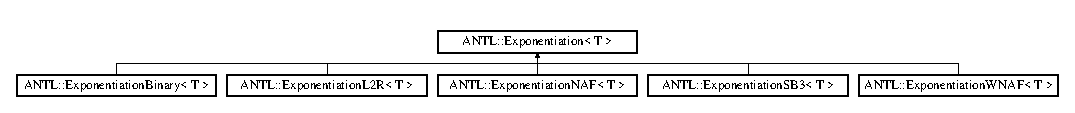
\includegraphics[height=2.000000cm]{dd/da0/classANTL_1_1Exponentiation}
\end{center}
\end{figure}
\subsection*{Public Member Functions}
\begin{DoxyCompactItemize}
\item 
virtual void \hyperlink{classANTL_1_1Exponentiation_aad4e3be9ab770361f04a10a85d390622}{power} (T \&C, const T \&A, const Z\-Z \&n)=0
\begin{DoxyCompactList}\small\item\em Computes A$^\wedge$n. Virtual method, to be overridden by concrete classes corresponding to different exponentiation methods. \end{DoxyCompactList}\end{DoxyCompactItemize}


\subsection{Detailed Description}
\subsubsection*{template$<$class T$>$class A\-N\-T\-L\-::\-Exponentiation$<$ T $>$}

Virtual superclass for generic exponentiation. 

\begin{DoxyRemark}{Remarks}
This virtual class defines a method for generic exponentiation. Particular exponentiation algorithms are defined and implemented in concrete subclasses. The base type is templated, and must have as a minimum the following functions defined\-:
\begin{DoxyItemize}
\item assign(\-T \&\-C, const T \&\-A)\-: sets C = A
\item mul(\-T \&\-C, const T \&\-A, const T \&\-B)\-: computes C = A\-B
\item sqr(\-T \&\-C, const T \&\-A)\-: computes C = A\-A Concrete subclasses may have further requirements (eg. a cube function) that are described in the documentation of each concrete class. 
\end{DoxyItemize}
\end{DoxyRemark}


\subsection{Member Function Documentation}
\hypertarget{classANTL_1_1Exponentiation_aad4e3be9ab770361f04a10a85d390622}{\index{A\-N\-T\-L\-::\-Exponentiation@{A\-N\-T\-L\-::\-Exponentiation}!power@{power}}
\index{power@{power}!ANTL::Exponentiation@{A\-N\-T\-L\-::\-Exponentiation}}
\subsubsection[{power}]{\setlength{\rightskip}{0pt plus 5cm}template$<$class T $>$ virtual void {\bf A\-N\-T\-L\-::\-Exponentiation}$<$ T $>$\-::power (
\begin{DoxyParamCaption}
\item[{T \&}]{C, }
\item[{const T \&}]{A, }
\item[{const Z\-Z \&}]{n}
\end{DoxyParamCaption}
)\hspace{0.3cm}{\ttfamily [pure virtual]}}}\label{classANTL_1_1Exponentiation_aad4e3be9ab770361f04a10a85d390622}


Computes A$^\wedge$n. Virtual method, to be overridden by concrete classes corresponding to different exponentiation methods. 


\begin{DoxyParams}[1]{Parameters}
\mbox{\tt out}  & {\em C} & result of computing A$^\wedge$n \\
\hline
\mbox{\tt in}  & {\em A} & base for exponentiation \\
\hline
\mbox{\tt in}  & {\em n} & exponent\\
\hline
\end{DoxyParams}
\begin{DoxyPrecond}{Precondition}
n $>$= 0 
\end{DoxyPrecond}


Implemented in \hyperlink{classANTL_1_1ExponentiationNAF_ae8d97318323ee8b3a888080d75f2cc39}{A\-N\-T\-L\-::\-Exponentiation\-N\-A\-F$<$ T $>$}, and \hyperlink{classANTL_1_1ExponentiationBinary_a039ea9d52144229d0728d81060d43fc4}{A\-N\-T\-L\-::\-Exponentiation\-Binary$<$ T $>$}.



The documentation for this class was generated from the following file\-:\begin{DoxyCompactItemize}
\item 
include/\-A\-N\-T\-L/\-Exponentiation/\hyperlink{Exponentiation_8hpp}{Exponentiation.\-hpp}\end{DoxyCompactItemize}

\hypertarget{classANTL_1_1ExponentiationBinary}{\section{A\-N\-T\-L\-:\-:Exponentiation\-Binary$<$ T $>$ Class Template Reference}
\label{classANTL_1_1ExponentiationBinary}\index{A\-N\-T\-L\-::\-Exponentiation\-Binary$<$ T $>$@{A\-N\-T\-L\-::\-Exponentiation\-Binary$<$ T $>$}}
}


class for left-\/to-\/right binary exponentiation  




{\ttfamily \#include $<$Exponentiation\-Binary.\-hpp$>$}

Inheritance diagram for A\-N\-T\-L\-:\-:Exponentiation\-Binary$<$ T $>$\-:\begin{figure}[H]
\begin{center}
\leavevmode
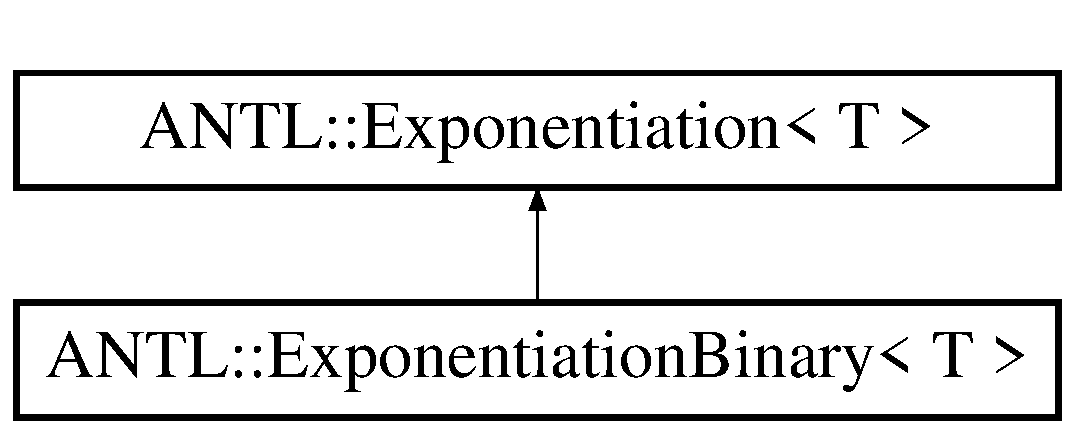
\includegraphics[height=2.000000cm]{d8/d7d/classANTL_1_1ExponentiationBinary}
\end{center}
\end{figure}
\subsection*{Public Member Functions}
\begin{DoxyCompactItemize}
\item 
void \hyperlink{classANTL_1_1ExponentiationBinary_a039ea9d52144229d0728d81060d43fc4}{power} (T \&C, const T \&A, const Z\-Z \&n)
\begin{DoxyCompactList}\small\item\em Computes A$^\wedge$n using left-\/to-\/right binary exponentiation. \end{DoxyCompactList}\end{DoxyCompactItemize}


\subsection{Detailed Description}
\subsubsection*{template$<$class T$>$class A\-N\-T\-L\-::\-Exponentiation\-Binary$<$ T $>$}

class for left-\/to-\/right binary exponentiation 

\begin{DoxyRemark}{Remarks}
This concrete class defines a method for standard left-\/to-\/right binary exponentiation. The base type is templated, and must have the following functions defined\-:
\begin{DoxyItemize}
\item assign(\-T \&\-C, const T \&\-A)\-: sets C = A
\item mul(\-T \&\-C, const T \&\-A, const T \&\-B)\-: computes C = A\-B
\item sqr(\-T \&\-C, const T \&\-A)\-: computes C = A\-A 
\end{DoxyItemize}
\end{DoxyRemark}


\subsection{Member Function Documentation}
\hypertarget{classANTL_1_1ExponentiationBinary_a039ea9d52144229d0728d81060d43fc4}{\index{A\-N\-T\-L\-::\-Exponentiation\-Binary@{A\-N\-T\-L\-::\-Exponentiation\-Binary}!power@{power}}
\index{power@{power}!ANTL::ExponentiationBinary@{A\-N\-T\-L\-::\-Exponentiation\-Binary}}
\subsubsection[{power}]{\setlength{\rightskip}{0pt plus 5cm}template$<$class T $>$ void Exponentiation\-Binary\-::power (
\begin{DoxyParamCaption}
\item[{T \&}]{C, }
\item[{const T \&}]{A, }
\item[{const Z\-Z \&}]{n}
\end{DoxyParamCaption}
)\hspace{0.3cm}{\ttfamily [virtual]}}}\label{classANTL_1_1ExponentiationBinary_a039ea9d52144229d0728d81060d43fc4}


Computes A$^\wedge$n using left-\/to-\/right binary exponentiation. 


\begin{DoxyParams}[1]{Parameters}
\mbox{\tt out}  & {\em C} & result of computing A$^\wedge$n \\
\hline
\mbox{\tt in}  & {\em A} & base for exponentiation \\
\hline
\mbox{\tt in}  & {\em n} & exponent\\
\hline
\end{DoxyParams}
\begin{DoxyPrecond}{Precondition}
n $>$= 0 
\end{DoxyPrecond}


Implements \hyperlink{classANTL_1_1Exponentiation_aad4e3be9ab770361f04a10a85d390622}{A\-N\-T\-L\-::\-Exponentiation$<$ T $>$}.



The documentation for this class was generated from the following files\-:\begin{DoxyCompactItemize}
\item 
include/\-A\-N\-T\-L/\-Exponentiation/\hyperlink{ExponentiationBinary_8hpp}{Exponentiation\-Binary.\-hpp}\item 
src/\-Exponentiation/\hyperlink{ExponentiationBinary__impl_8hpp}{Exponentiation\-Binary\-\_\-impl.\-hpp}\end{DoxyCompactItemize}

\hypertarget{classANTL_1_1ExponentiationNAF}{\section{A\-N\-T\-L\-:\-:Exponentiation\-N\-A\-F$<$ T $>$ Class Template Reference}
\label{classANTL_1_1ExponentiationNAF}\index{A\-N\-T\-L\-::\-Exponentiation\-N\-A\-F$<$ T $>$@{A\-N\-T\-L\-::\-Exponentiation\-N\-A\-F$<$ T $>$}}
}


class for left-\/to-\/right N\-A\-F exponentiation  




{\ttfamily \#include $<$Exponentiation\-N\-A\-F.\-hpp$>$}

Inheritance diagram for A\-N\-T\-L\-:\-:Exponentiation\-N\-A\-F$<$ T $>$\-:\begin{figure}[H]
\begin{center}
\leavevmode
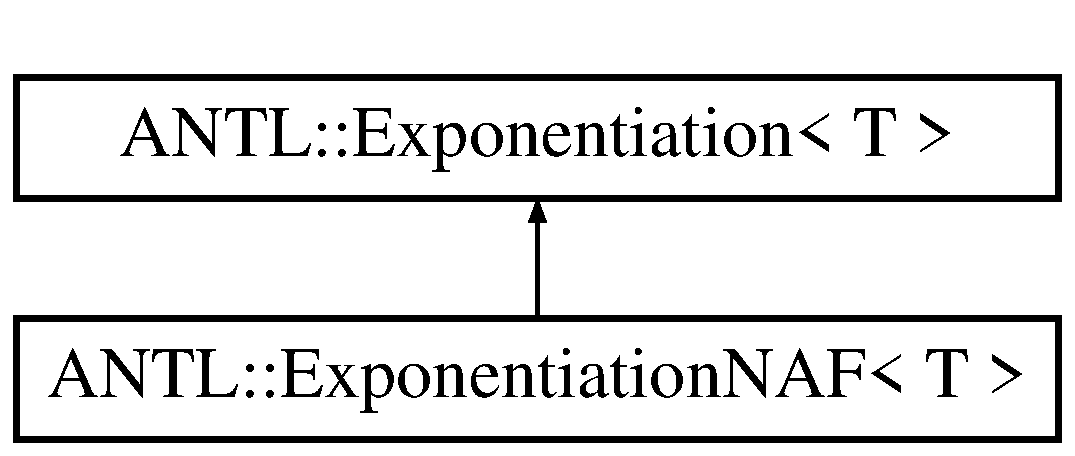
\includegraphics[height=2.000000cm]{db/d6c/classANTL_1_1ExponentiationNAF}
\end{center}
\end{figure}
\subsection*{Public Member Functions}
\begin{DoxyCompactItemize}
\item 
void \hyperlink{classANTL_1_1ExponentiationNAF_aa70b6e1083b3936ed0a234998624a188}{initialize} (const T \&A, const Z\-Z \&n)
\begin{DoxyCompactList}\small\item\em Setup the class to compute A$^\wedge$n. Compute inverse of A and allocates a digit vector of size Num\-Bits(n)+1. \end{DoxyCompactList}\item 
void \hyperlink{classANTL_1_1ExponentiationNAF_ae8d97318323ee8b3a888080d75f2cc39}{power} (T \&C, const T \&A, const Z\-Z \&n)
\begin{DoxyCompactList}\small\item\em Computes A$^\wedge$n. \end{DoxyCompactList}\end{DoxyCompactItemize}
\subsection*{Protected Attributes}
\begin{DoxyCompactItemize}
\item 
vector$<$ short $>$ \hyperlink{classANTL_1_1ExponentiationNAF_a9cbe814c668d82453284afc1f662e3e2}{e}
\item 
T \hyperlink{classANTL_1_1ExponentiationNAF_a3daf8a194f65ea69e18882e03e2d9af7}{Ainv}
\end{DoxyCompactItemize}


\subsection{Detailed Description}
\subsubsection*{template$<$class T$>$class A\-N\-T\-L\-::\-Exponentiation\-N\-A\-F$<$ T $>$}

class for left-\/to-\/right N\-A\-F exponentiation 

\begin{DoxyRemark}{Remarks}
This concrete class defines a method for left-\/to-\/right non-\/adjacent form exponentiation. The method first computes the N\-A\-F representation of the exponent using the basic right-\/to-\/left method, and then applies it to the base left-\/to-\/right. The base type is templated, and must have the following functions defined\-:
\begin{DoxyItemize}
\item assign(\-T \&\-C, const T \&\-A)\-: sets C = A
\item mul(\-T \&\-C, const T \&\-A, const T \&\-B)\-: computes C = A\-B
\item sqr(\-T \&\-C, const T \&\-A)\-: computes C = A\-A
\item inv(\-T \&\-C, const T \&\-A)\-: computes C = inverse of A 
\end{DoxyItemize}
\end{DoxyRemark}


\subsection{Member Function Documentation}
\hypertarget{classANTL_1_1ExponentiationNAF_aa70b6e1083b3936ed0a234998624a188}{\index{A\-N\-T\-L\-::\-Exponentiation\-N\-A\-F@{A\-N\-T\-L\-::\-Exponentiation\-N\-A\-F}!initialize@{initialize}}
\index{initialize@{initialize}!ANTL::ExponentiationNAF@{A\-N\-T\-L\-::\-Exponentiation\-N\-A\-F}}
\subsubsection[{initialize}]{\setlength{\rightskip}{0pt plus 5cm}template$<$class T $>$ void Exponentiation\-N\-A\-F\-::initialize (
\begin{DoxyParamCaption}
\item[{const T \&}]{A, }
\item[{const Z\-Z \&}]{n}
\end{DoxyParamCaption}
)}}\label{classANTL_1_1ExponentiationNAF_aa70b6e1083b3936ed0a234998624a188}


Setup the class to compute A$^\wedge$n. Compute inverse of A and allocates a digit vector of size Num\-Bits(n)+1. 


\begin{DoxyParams}[1]{Parameters}
\mbox{\tt in}  & {\em A} & base for exponentiation \\
\hline
\mbox{\tt in}  & {\em n} & exponent\\
\hline
\end{DoxyParams}
\begin{DoxyPrecond}{Precondition}
n $>$= 0 
\end{DoxyPrecond}
\hypertarget{classANTL_1_1ExponentiationNAF_ae8d97318323ee8b3a888080d75f2cc39}{\index{A\-N\-T\-L\-::\-Exponentiation\-N\-A\-F@{A\-N\-T\-L\-::\-Exponentiation\-N\-A\-F}!power@{power}}
\index{power@{power}!ANTL::ExponentiationNAF@{A\-N\-T\-L\-::\-Exponentiation\-N\-A\-F}}
\subsubsection[{power}]{\setlength{\rightskip}{0pt plus 5cm}template$<$class T $>$ void Exponentiation\-N\-A\-F\-::power (
\begin{DoxyParamCaption}
\item[{T \&}]{C, }
\item[{const T \&}]{A, }
\item[{const Z\-Z \&}]{n}
\end{DoxyParamCaption}
)\hspace{0.3cm}{\ttfamily [virtual]}}}\label{classANTL_1_1ExponentiationNAF_ae8d97318323ee8b3a888080d75f2cc39}


Computes A$^\wedge$n. 


\begin{DoxyParams}[1]{Parameters}
\mbox{\tt out}  & {\em C} & result of computing A$^\wedge$n using left-\/to-\/right N\-A\-F exponentiation \\
\hline
\mbox{\tt in}  & {\em A} & base for exponentiation \\
\hline
\mbox{\tt in}  & {\em n} & exponent\\
\hline
\end{DoxyParams}
\begin{DoxyPrecond}{Precondition}
n $>$= 0 
\end{DoxyPrecond}


Implements \hyperlink{classANTL_1_1Exponentiation_aad4e3be9ab770361f04a10a85d390622}{A\-N\-T\-L\-::\-Exponentiation$<$ T $>$}.



\subsection{Member Data Documentation}
\hypertarget{classANTL_1_1ExponentiationNAF_a3daf8a194f65ea69e18882e03e2d9af7}{\index{A\-N\-T\-L\-::\-Exponentiation\-N\-A\-F@{A\-N\-T\-L\-::\-Exponentiation\-N\-A\-F}!Ainv@{Ainv}}
\index{Ainv@{Ainv}!ANTL::ExponentiationNAF@{A\-N\-T\-L\-::\-Exponentiation\-N\-A\-F}}
\subsubsection[{Ainv}]{\setlength{\rightskip}{0pt plus 5cm}template$<$class T $>$ T {\bf A\-N\-T\-L\-::\-Exponentiation\-N\-A\-F}$<$ T $>$\-::Ainv\hspace{0.3cm}{\ttfamily [protected]}}}\label{classANTL_1_1ExponentiationNAF_a3daf8a194f65ea69e18882e03e2d9af7}
inverse of the base element \hypertarget{classANTL_1_1ExponentiationNAF_a9cbe814c668d82453284afc1f662e3e2}{\index{A\-N\-T\-L\-::\-Exponentiation\-N\-A\-F@{A\-N\-T\-L\-::\-Exponentiation\-N\-A\-F}!e@{e}}
\index{e@{e}!ANTL::ExponentiationNAF@{A\-N\-T\-L\-::\-Exponentiation\-N\-A\-F}}
\subsubsection[{e}]{\setlength{\rightskip}{0pt plus 5cm}template$<$class T $>$ vector$<$short$>$ {\bf A\-N\-T\-L\-::\-Exponentiation\-N\-A\-F}$<$ T $>$\-::e\hspace{0.3cm}{\ttfamily [protected]}}}\label{classANTL_1_1ExponentiationNAF_a9cbe814c668d82453284afc1f662e3e2}
vector containing N\-A\-F expansion of exponent 

The documentation for this class was generated from the following files\-:\begin{DoxyCompactItemize}
\item 
include/\-A\-N\-T\-L/\-Exponentiation/\hyperlink{ExponentiationNAF_8hpp}{Exponentiation\-N\-A\-F.\-hpp}\item 
src/\-Exponentiation/\hyperlink{ExponentiationNAF__impl_8hpp}{Exponentiation\-N\-A\-F\-\_\-impl.\-hpp}\end{DoxyCompactItemize}

\hypertarget{classANTL_1_1nullbuf}{\section{A\-N\-T\-L\-:\-:nullbuf Class Reference}
\label{classANTL_1_1nullbuf}\index{A\-N\-T\-L\-::nullbuf@{A\-N\-T\-L\-::nullbuf}}
}
Inheritance diagram for A\-N\-T\-L\-:\-:nullbuf\-:\begin{figure}[H]
\begin{center}
\leavevmode
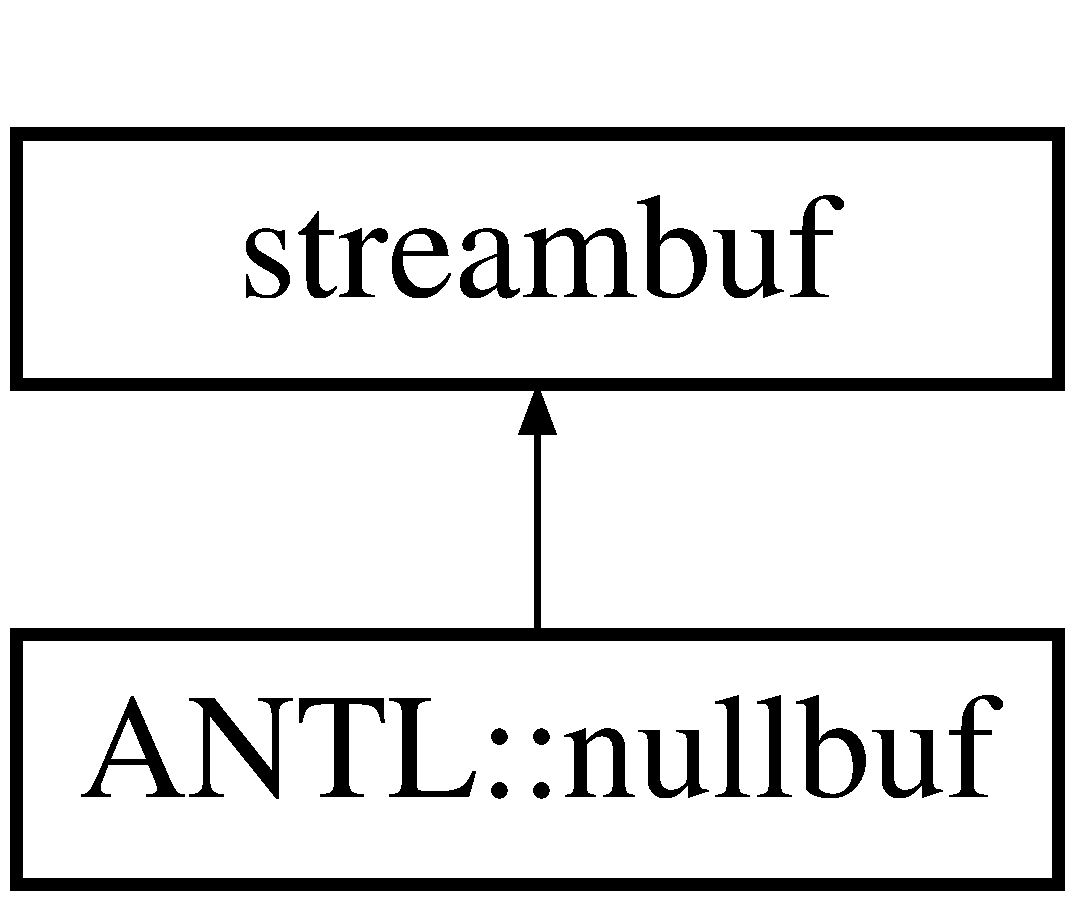
\includegraphics[height=2.000000cm]{d9/ddf/classANTL_1_1nullbuf}
\end{center}
\end{figure}
\subsection*{Public Member Functions}
\begin{DoxyCompactItemize}
\item 
\hypertarget{classANTL_1_1nullbuf_a535cf51861da38ddc0214972cd99de08}{int\-\_\-type {\bfseries overflow} (int\-\_\-type c)}\label{classANTL_1_1nullbuf_a535cf51861da38ddc0214972cd99de08}

\end{DoxyCompactItemize}


\subsection{Detailed Description}
Mechanism for a streambuf that creates a stream that does nothing. 

The documentation for this class was generated from the following file\-:\begin{DoxyCompactItemize}
\item 
src/\hyperlink{debug_8cpp}{debug.\-cpp}\end{DoxyCompactItemize}

\chapter{File Documentation}
\hypertarget{common_8hpp}{\section{include/\-A\-N\-T\-L/common.hpp File Reference}
\label{common_8hpp}\index{include/\-A\-N\-T\-L/common.\-hpp@{include/\-A\-N\-T\-L/common.\-hpp}}
}


General-\/purpose methods to interface with N\-T\-L. All library files should include this file.  


{\ttfamily \#include $<$cmath$>$}\\*
{\ttfamily \#include $<$N\-T\-L/\-Z\-Z.\-h$>$}\\*
{\ttfamily \#include $<$N\-T\-L/\-R\-R.\-h$>$}\\*
{\ttfamily \#include $<$N\-T\-L/\-G\-F2\-E\-X.\-h$>$}\\*
{\ttfamily \#include $<$N\-T\-L/\-Z\-Z\-\_\-p\-X.\-h$>$}\\*
{\ttfamily \#include $<$N\-T\-L/lzz\-\_\-p\-X.\-h$>$}\\*
{\ttfamily \#include $<$N\-T\-L/\-Z\-Z\-\_\-p\-E\-X.\-h$>$}\\*
{\ttfamily \#include $<$N\-T\-L/lzz\-\_\-p\-E\-X.\-h$>$}\\*
{\ttfamily \#include \char`\"{}debug.\-hpp\char`\"{}}\\*
\subsection*{Macros}
\begin{DoxyCompactItemize}
\item 
\#define \hyperlink{common_8hpp_a2434fc9dd1b385585ccbdfd840bc327a}{A\-N\-T\-L\-\_\-\-B\-E\-G\-I\-N\-\_\-\-M\-A\-C\-R\-O\-\_\-\-F\-U\-N\-C\-T\-I\-O\-N}~do \{
\begin{DoxyCompactList}\small\item\em Suggested beginning of the definition of a function-\/like macro. \end{DoxyCompactList}\item 
\hypertarget{common_8hpp_acb4b3218c4498189f6afd9fb235f7568}{\#define \hyperlink{common_8hpp_acb4b3218c4498189f6afd9fb235f7568}{A\-N\-T\-L\-\_\-\-E\-N\-D\-\_\-\-M\-A\-C\-R\-O\-\_\-\-F\-U\-N\-C\-T\-I\-O\-N}~\} while(0)}\label{common_8hpp_acb4b3218c4498189f6afd9fb235f7568}

\begin{DoxyCompactList}\small\item\em Used to close a macro definition started with {\ttfamily A\-N\-T\-L\-\_\-\-B\-E\-G\-I\-N\-\_\-\-M\-A\-C\-R\-O}. \end{DoxyCompactList}\item 
\#define \hyperlink{common_8hpp_aa3b633c1a963f8868f44e8fc27904649}{R\-E\-F}
\begin{DoxyCompactList}\small\item\em Null macro used to mark a by-\/reference argument pass. \end{DoxyCompactList}\end{DoxyCompactItemize}
\subsection*{Functions}
\begin{DoxyCompactItemize}
\item 
\hypertarget{namespaceNTL_accb9e562ed1d5c776d163f611183f7c4}{void {\bfseries N\-T\-L\-::clear} (long \&X)}\label{namespaceNTL_accb9e562ed1d5c776d163f611183f7c4}

\item 
\hypertarget{namespaceNTL_afff7a3b929e0b072710e29e250144948}{void {\bfseries N\-T\-L\-::set} (long \&X)}\label{namespaceNTL_afff7a3b929e0b072710e29e250144948}

\item 
\hypertarget{namespaceNTL_a483059ceccb8be02108e7eaf5133e850}{void {\bfseries N\-T\-L\-::clear} (float \&i)}\label{namespaceNTL_a483059ceccb8be02108e7eaf5133e850}

\item 
\hypertarget{namespaceNTL_af91c4b216325e29153bbaf242bc9f9f4}{void {\bfseries N\-T\-L\-::set} (float \&i)}\label{namespaceNTL_af91c4b216325e29153bbaf242bc9f9f4}

\item 
\hypertarget{namespaceNTL_ad847d4245f1df6ed8ea0387f8c3d5ac6}{void {\bfseries N\-T\-L\-::clear} (double \&i)}\label{namespaceNTL_ad847d4245f1df6ed8ea0387f8c3d5ac6}

\item 
\hypertarget{namespaceNTL_afb42e095bdf60dd963c64e8befa9cdec}{void {\bfseries N\-T\-L\-::set} (double \&i)}\label{namespaceNTL_afb42e095bdf60dd963c64e8befa9cdec}

\item 
\hypertarget{namespaceNTL_a8265e0aeaea089dc03b19c808b44270f}{void {\bfseries N\-T\-L\-::clear} (quad\-\_\-float \&i)}\label{namespaceNTL_a8265e0aeaea089dc03b19c808b44270f}

\item 
\hypertarget{namespaceNTL_a10ebe5a15ce87a433f2be2f9382b94fd}{void {\bfseries N\-T\-L\-::set} (quad\-\_\-float \&i)}\label{namespaceNTL_a10ebe5a15ce87a433f2be2f9382b94fd}

\item 
\hypertarget{namespaceNTL_af0756583d985819face121a13f8278e2}{long {\bfseries N\-T\-L\-::\-Is\-One} (const long \&X)}\label{namespaceNTL_af0756583d985819face121a13f8278e2}

\item 
\hypertarget{namespaceNTL_ab1e2294e90f75960987add5a755d1757}{long {\bfseries N\-T\-L\-::\-Is\-Zero} (const long \&X)}\label{namespaceNTL_ab1e2294e90f75960987add5a755d1757}

\item 
\hypertarget{namespaceNTL_a72fc72ad3aa50379ef6d819441486abc}{long {\bfseries N\-T\-L\-::\-Is\-Odd} (const long \&X)}\label{namespaceNTL_a72fc72ad3aa50379ef6d819441486abc}

\item 
\hypertarget{namespaceNTL_a6530c2adbfdf6f9c32fbc009e4666387}{long {\bfseries N\-T\-L\-::\-Is\-One} (const float \&X)}\label{namespaceNTL_a6530c2adbfdf6f9c32fbc009e4666387}

\item 
\hypertarget{namespaceNTL_a66d0bc269e79c0f82e7efbc04a757239}{long {\bfseries N\-T\-L\-::\-Is\-Zero} (const float \&X)}\label{namespaceNTL_a66d0bc269e79c0f82e7efbc04a757239}

\item 
\hypertarget{namespaceNTL_a0d4a3b717be78ace5c1e586eb27b79c6}{long {\bfseries N\-T\-L\-::\-Is\-One} (const double \&X)}\label{namespaceNTL_a0d4a3b717be78ace5c1e586eb27b79c6}

\item 
\hypertarget{namespaceNTL_accbf2d629df06bab285d322346fbae80}{long {\bfseries N\-T\-L\-::\-Is\-Zero} (const double \&X)}\label{namespaceNTL_accbf2d629df06bab285d322346fbae80}

\item 
\hypertarget{namespaceNTL_a1ce2809542ad1e4294a1ee94731c2796}{long {\bfseries N\-T\-L\-::\-Is\-One} (const quad\-\_\-float \&X)}\label{namespaceNTL_a1ce2809542ad1e4294a1ee94731c2796}

\item 
\hypertarget{namespaceNTL_ac09334675386e8f21fb411350f236f76}{long {\bfseries N\-T\-L\-::\-Is\-Zero} (const quad\-\_\-float \&X)}\label{namespaceNTL_ac09334675386e8f21fb411350f236f76}

\item 
\hypertarget{namespaceNTL_aeee609c03ad8d69c4a8dccaf864066bb}{long {\bfseries N\-T\-L\-::deg} (long X)}\label{namespaceNTL_aeee609c03ad8d69c4a8dccaf864066bb}

\item 
\hypertarget{namespaceNTL_a284fd034213467bf7dbb57fc604ee299}{long {\bfseries N\-T\-L\-::deg} (const Z\-Z \&X)}\label{namespaceNTL_a284fd034213467bf7dbb57fc604ee299}

\item 
\hypertarget{namespaceNTL_a51b43b879b277eed4dfe3a89af231569}{long {\bfseries N\-T\-L\-::\-Lead\-Coeff} (long X)}\label{namespaceNTL_a51b43b879b277eed4dfe3a89af231569}

\item 
\hypertarget{namespaceNTL_a147eaf20e47e437f528c2cca78ea1c61}{Z\-Z {\bfseries N\-T\-L\-::\-Lead\-Coeff} (const Z\-Z \&X)}\label{namespaceNTL_a147eaf20e47e437f528c2cca78ea1c61}

\item 
\hypertarget{namespaceNTL_a90af800362efbfc0e0ff10cfdc401d6f}{void {\bfseries N\-T\-L\-::\-Make\-Monic} (long \&X)}\label{namespaceNTL_a90af800362efbfc0e0ff10cfdc401d6f}

\item 
\hypertarget{namespaceNTL_ae3b95df8da6c33b005f4a37f34dd4a8c}{void {\bfseries N\-T\-L\-::\-Make\-Monic} (Z\-Z \&X)}\label{namespaceNTL_ae3b95df8da6c33b005f4a37f34dd4a8c}

\item 
\hypertarget{namespaceNTL_a4729a044c1c8f9db680e28d5d0b454a9}{{\footnotesize template$<$class T $>$ }\\void {\bfseries N\-T\-L\-::assign} (T \&C, const T \&A)}\label{namespaceNTL_a4729a044c1c8f9db680e28d5d0b454a9}

\item 
\hypertarget{namespaceANTL_a02a5f61db8f020d498eb2e6586083b2d}{int {\bfseries A\-N\-T\-L\-::\-Sqr\-Root} (const int \&a)}\label{namespaceANTL_a02a5f61db8f020d498eb2e6586083b2d}

\item 
\hypertarget{namespaceANTL_ac30856c0e33c55bf08c1d14146b1b7a1}{void {\bfseries A\-N\-T\-L\-::\-Div\-Rem} (long \&q, long \&r, long a, long b)}\label{namespaceANTL_ac30856c0e33c55bf08c1d14146b1b7a1}

\item 
\hypertarget{namespaceANTL_a01ab42bbe002693705cee888d3fdd244}{long {\bfseries A\-N\-T\-L\-::\-Sqr\-Root} (const long \&a)}\label{namespaceANTL_a01ab42bbe002693705cee888d3fdd244}

\item 
\hypertarget{namespaceANTL_a6fe2e55cd9263c2addfb027e7cc89666}{float {\bfseries A\-N\-T\-L\-::sqrt} (float x)}\label{namespaceANTL_a6fe2e55cd9263c2addfb027e7cc89666}

\item 
\hypertarget{namespaceANTL_a308aa1f1eb671675b904dafc45a13982}{double {\bfseries A\-N\-T\-L\-::sqrt} (double x)}\label{namespaceANTL_a308aa1f1eb671675b904dafc45a13982}

\item 
\hypertarget{namespaceANTL_a1b4361c41c5dd6224e309cec3a36b46f}{long {\bfseries A\-N\-T\-L\-::abs} (long x)}\label{namespaceANTL_a1b4361c41c5dd6224e309cec3a36b46f}

\item 
\hypertarget{namespaceANTL_ad588f69d817ad6e7e035b78e48231957}{float {\bfseries A\-N\-T\-L\-::abs} (float x)}\label{namespaceANTL_ad588f69d817ad6e7e035b78e48231957}

\item 
\hypertarget{namespaceANTL_aa92540de499f038e66ef018fb0cd0a33}{double {\bfseries A\-N\-T\-L\-::abs} (double x)}\label{namespaceANTL_aa92540de499f038e66ef018fb0cd0a33}

\item 
\hypertarget{namespaceANTL_a025db022bb86f1dba3ede198e4a47376}{quad\-\_\-float {\bfseries A\-N\-T\-L\-::abs} (const quad\-\_\-float \&x)}\label{namespaceANTL_a025db022bb86f1dba3ede198e4a47376}

\item 
\hypertarget{namespaceANTL_a66702f96702b1d5533ef17a3034b6284}{float {\bfseries A\-N\-T\-L\-::exp} (float x)}\label{namespaceANTL_a66702f96702b1d5533ef17a3034b6284}

\item 
\hypertarget{namespaceANTL_adabb25cd3ed8202bb6f4e970b65c42b1}{double {\bfseries A\-N\-T\-L\-::exp} (double x)}\label{namespaceANTL_adabb25cd3ed8202bb6f4e970b65c42b1}

\item 
\hypertarget{namespaceANTL_a767b92b7b3705bec4c613f60a1199fc6}{float {\bfseries A\-N\-T\-L\-::log} (float x)}\label{namespaceANTL_a767b92b7b3705bec4c613f60a1199fc6}

\item 
\hypertarget{namespaceANTL_a7337d1395d7a25fa51127f60a0bfe760}{double {\bfseries A\-N\-T\-L\-::log} (double x)}\label{namespaceANTL_a7337d1395d7a25fa51127f60a0bfe760}

\item 
\hypertarget{namespaceANTL_a5c76a56114b86a1b57a8b2429a301285}{{\footnotesize template$<$class $>$ }\\Z\-Z {\bfseries A\-N\-T\-L\-::\-C\-A\-R\-D\-I\-N\-A\-L\-I\-T\-Y} (void)}\label{namespaceANTL_a5c76a56114b86a1b57a8b2429a301285}

\item 
\hypertarget{namespaceANTL_a987cb941416d193c52607244e20e5817}{{\footnotesize template$<$$>$ }\\Z\-Z {\bfseries A\-N\-T\-L\-::\-C\-A\-R\-D\-I\-N\-A\-L\-I\-T\-Y$<$ Z\-Z $>$} (void)}\label{namespaceANTL_a987cb941416d193c52607244e20e5817}

\item 
\hypertarget{namespaceANTL_a9516296216e3890465962e20371bccee}{{\footnotesize template$<$$>$ }\\Z\-Z {\bfseries A\-N\-T\-L\-::\-C\-A\-R\-D\-I\-N\-A\-L\-I\-T\-Y$<$ long $>$} (void)}\label{namespaceANTL_a9516296216e3890465962e20371bccee}

\item 
\hypertarget{namespaceANTL_aebe9002acf012122eb897adeb31502d2}{{\footnotesize template$<$$>$ }\\Z\-Z {\bfseries A\-N\-T\-L\-::\-C\-A\-R\-D\-I\-N\-A\-L\-I\-T\-Y$<$ Z\-Z\-\_\-p $>$} (void)}\label{namespaceANTL_aebe9002acf012122eb897adeb31502d2}

\item 
\hypertarget{namespaceANTL_a64544fa2eb7c272fed1f5df936d2946b}{{\footnotesize template$<$$>$ }\\Z\-Z {\bfseries A\-N\-T\-L\-::\-C\-A\-R\-D\-I\-N\-A\-L\-I\-T\-Y$<$ zz\-\_\-p $>$} (void)}\label{namespaceANTL_a64544fa2eb7c272fed1f5df936d2946b}

\item 
\hypertarget{namespaceANTL_a6afc32e10d36b5f4a8c01ac00b6914f2}{{\footnotesize template$<$$>$ }\\Z\-Z {\bfseries A\-N\-T\-L\-::\-C\-A\-R\-D\-I\-N\-A\-L\-I\-T\-Y$<$ Z\-Z\-\_\-p\-X $>$} (void)}\label{namespaceANTL_a6afc32e10d36b5f4a8c01ac00b6914f2}

\item 
\hypertarget{namespaceANTL_ab4142fdaaec089efc5f8a3afbdf69ad2}{{\footnotesize template$<$$>$ }\\Z\-Z {\bfseries A\-N\-T\-L\-::\-C\-A\-R\-D\-I\-N\-A\-L\-I\-T\-Y$<$ zz\-\_\-p\-X $>$} (void)}\label{namespaceANTL_ab4142fdaaec089efc5f8a3afbdf69ad2}

\item 
\hypertarget{namespaceANTL_a86cd8dd0cc9927427d822a73d5cae946}{{\footnotesize template$<$$>$ }\\Z\-Z {\bfseries A\-N\-T\-L\-::\-C\-A\-R\-D\-I\-N\-A\-L\-I\-T\-Y$<$ Z\-Z\-\_\-p\-E $>$} (void)}\label{namespaceANTL_a86cd8dd0cc9927427d822a73d5cae946}

\item 
\hypertarget{namespaceANTL_a9b528e0c099767a016a7ff1b9a67c971}{{\footnotesize template$<$$>$ }\\Z\-Z {\bfseries A\-N\-T\-L\-::\-C\-A\-R\-D\-I\-N\-A\-L\-I\-T\-Y$<$ zz\-\_\-p\-E $>$} (void)}\label{namespaceANTL_a9b528e0c099767a016a7ff1b9a67c971}

\item 
\hypertarget{namespaceANTL_aa811f1868565af5d989a48bf6c1a140d}{{\footnotesize template$<$$>$ }\\Z\-Z {\bfseries A\-N\-T\-L\-::\-C\-A\-R\-D\-I\-N\-A\-L\-I\-T\-Y$<$ Z\-Z\-\_\-p\-E\-X $>$} (void)}\label{namespaceANTL_aa811f1868565af5d989a48bf6c1a140d}

\item 
\hypertarget{namespaceANTL_a60cab2907bca8671895078c96de17da9}{{\footnotesize template$<$$>$ }\\Z\-Z {\bfseries A\-N\-T\-L\-::\-C\-A\-R\-D\-I\-N\-A\-L\-I\-T\-Y$<$ zz\-\_\-p\-E\-X $>$} (void)}\label{namespaceANTL_a60cab2907bca8671895078c96de17da9}

\item 
\hypertarget{namespaceANTL_a75b01f509ada118f056ab8075349f9cd}{{\footnotesize template$<$$>$ }\\Z\-Z {\bfseries A\-N\-T\-L\-::\-C\-A\-R\-D\-I\-N\-A\-L\-I\-T\-Y$<$ G\-F2\-E $>$} (void)}\label{namespaceANTL_a75b01f509ada118f056ab8075349f9cd}

\item 
\hypertarget{namespaceANTL_a1f26ef340fea6680888990863640d46b}{{\footnotesize template$<$$>$ }\\Z\-Z {\bfseries A\-N\-T\-L\-::\-C\-A\-R\-D\-I\-N\-A\-L\-I\-T\-Y$<$ G\-F2\-E\-X $>$} (void)}\label{namespaceANTL_a1f26ef340fea6680888990863640d46b}

\item 
\hypertarget{namespaceANTL_a5620caf50a40b13e80e1ba5ca5740bf6}{{\footnotesize template$<$class T $>$ }\\T {\bfseries A\-N\-T\-L\-::to} (const int \&a)}\label{namespaceANTL_a5620caf50a40b13e80e1ba5ca5740bf6}

\item 
\hypertarget{namespaceANTL_a00cf74fbb1ed8bfe8cfa66eb629da731}{{\footnotesize template$<$class T $>$ }\\T {\bfseries A\-N\-T\-L\-::to} (const long \&a)}\label{namespaceANTL_a00cf74fbb1ed8bfe8cfa66eb629da731}

\item 
\hypertarget{namespaceANTL_a55eb0a15934d8eb09f79e20d995082b1}{{\footnotesize template$<$class T $>$ }\\T {\bfseries A\-N\-T\-L\-::to} (const float \&a)}\label{namespaceANTL_a55eb0a15934d8eb09f79e20d995082b1}

\item 
\hypertarget{namespaceANTL_a1ca91e06bd4ddd48a995cc618d508b0e}{{\footnotesize template$<$class T $>$ }\\T {\bfseries A\-N\-T\-L\-::to} (const double \&a)}\label{namespaceANTL_a1ca91e06bd4ddd48a995cc618d508b0e}

\item 
\hypertarget{namespaceANTL_a8927b00cbebd8aa337714c271877d558}{{\footnotesize template$<$class T $>$ }\\T {\bfseries A\-N\-T\-L\-::to} (const Z\-Z \&a)}\label{namespaceANTL_a8927b00cbebd8aa337714c271877d558}

\item 
\hypertarget{namespaceANTL_a0ab25b680bbc5515f1845308d86991a3}{{\footnotesize template$<$class T $>$ }\\T {\bfseries A\-N\-T\-L\-::to} (const R\-R \&a)}\label{namespaceANTL_a0ab25b680bbc5515f1845308d86991a3}

\item 
\hypertarget{namespaceANTL_a265e8b791c640283b986013c49058d8e}{{\footnotesize template$<$class T $>$ }\\T {\bfseries A\-N\-T\-L\-::to} (const quad\-\_\-float \&a)}\label{namespaceANTL_a265e8b791c640283b986013c49058d8e}

\item 
\hypertarget{namespaceANTL_ae853eab087d691a39e217303055165f7}{{\footnotesize template$<$class T $>$ }\\T {\bfseries A\-N\-T\-L\-::to} (const G\-F2\-E\-X \&a)}\label{namespaceANTL_ae853eab087d691a39e217303055165f7}

\item 
\hypertarget{namespaceANTL_a3894196d836ce2c5dbfd0924f9692bd5}{{\footnotesize template$<$class T $>$ }\\T {\bfseries A\-N\-T\-L\-::to} (const zz\-\_\-p\-X \&a)}\label{namespaceANTL_a3894196d836ce2c5dbfd0924f9692bd5}

\item 
\hypertarget{namespaceANTL_a78b71f10516ebbca0a6e0903a41a7f08}{{\footnotesize template$<$class T $>$ }\\T {\bfseries A\-N\-T\-L\-::to} (const Z\-Z\-\_\-p\-X \&a)}\label{namespaceANTL_a78b71f10516ebbca0a6e0903a41a7f08}

\item 
\hypertarget{namespaceANTL_a4f7a4184e4a3f8e804956c1ad9863700}{{\footnotesize template$<$class T $>$ }\\T {\bfseries A\-N\-T\-L\-::to} (const zz\-\_\-p\-E\-X \&a)}\label{namespaceANTL_a4f7a4184e4a3f8e804956c1ad9863700}

\item 
\hypertarget{namespaceANTL_a271df7954c79470ffd281c08cbe79133}{{\footnotesize template$<$class T $>$ }\\T {\bfseries A\-N\-T\-L\-::to} (const Z\-Z\-\_\-p\-E\-X \&a)}\label{namespaceANTL_a271df7954c79470ffd281c08cbe79133}

\item 
\hypertarget{namespaceANTL_ad09486c547d98b412e2d1d3dd554dd38}{{\footnotesize template$<$$>$ }\\int {\bfseries A\-N\-T\-L\-::to$<$ int $>$} (const int \&a)}\label{namespaceANTL_ad09486c547d98b412e2d1d3dd554dd38}

\item 
\hypertarget{namespaceANTL_a17d8384a8348ad6dee43a44e78a546f9}{{\footnotesize template$<$$>$ }\\int {\bfseries A\-N\-T\-L\-::to$<$ int $>$} (const long \&a)}\label{namespaceANTL_a17d8384a8348ad6dee43a44e78a546f9}

\item 
\hypertarget{namespaceANTL_ac1bb93fbe57b6a78d689d7f12e39590e}{{\footnotesize template$<$$>$ }\\int {\bfseries A\-N\-T\-L\-::to$<$ int $>$} (const float \&a)}\label{namespaceANTL_ac1bb93fbe57b6a78d689d7f12e39590e}

\item 
\hypertarget{namespaceANTL_aec7dbf8402c8b45d4eb47eb9c7fda126}{{\footnotesize template$<$$>$ }\\int {\bfseries A\-N\-T\-L\-::to$<$ int $>$} (const double \&a)}\label{namespaceANTL_aec7dbf8402c8b45d4eb47eb9c7fda126}

\item 
\hypertarget{namespaceANTL_aac5f8a9b5abf76ea7aad0a13914d3c88}{{\footnotesize template$<$$>$ }\\int {\bfseries A\-N\-T\-L\-::to$<$ int $>$} (const Z\-Z \&a)}\label{namespaceANTL_aac5f8a9b5abf76ea7aad0a13914d3c88}

\item 
\hypertarget{namespaceANTL_a253755ab13595fb15a90d9a9c8d7a9d1}{{\footnotesize template$<$$>$ }\\int {\bfseries A\-N\-T\-L\-::to$<$ int $>$} (const R\-R \&a)}\label{namespaceANTL_a253755ab13595fb15a90d9a9c8d7a9d1}

\item 
\hypertarget{namespaceANTL_af7d76f98bbd3edc13daefcf2fb82f6aa}{{\footnotesize template$<$$>$ }\\int {\bfseries A\-N\-T\-L\-::to$<$ int $>$} (const quad\-\_\-float \&a)}\label{namespaceANTL_af7d76f98bbd3edc13daefcf2fb82f6aa}

\item 
\hypertarget{namespaceANTL_ade59a94c63bb2f5b6957e5626632dd19}{{\footnotesize template$<$$>$ }\\long {\bfseries A\-N\-T\-L\-::to$<$ long $>$} (const int \&a)}\label{namespaceANTL_ade59a94c63bb2f5b6957e5626632dd19}

\item 
\hypertarget{namespaceANTL_a958b355cfe166556117de5c656cf46fa}{{\footnotesize template$<$$>$ }\\long {\bfseries A\-N\-T\-L\-::to$<$ long $>$} (const long \&a)}\label{namespaceANTL_a958b355cfe166556117de5c656cf46fa}

\item 
\hypertarget{namespaceANTL_a5c62f4adb1ef863b891d2c02780cfb1c}{{\footnotesize template$<$$>$ }\\long {\bfseries A\-N\-T\-L\-::to$<$ long $>$} (const float \&a)}\label{namespaceANTL_a5c62f4adb1ef863b891d2c02780cfb1c}

\item 
\hypertarget{namespaceANTL_a2def72a7a6e4a0bffa2578dec32f40bb}{{\footnotesize template$<$$>$ }\\long {\bfseries A\-N\-T\-L\-::to$<$ long $>$} (const double \&a)}\label{namespaceANTL_a2def72a7a6e4a0bffa2578dec32f40bb}

\item 
\hypertarget{namespaceANTL_a2142984e3d5eac9b07410d469d18355b}{{\footnotesize template$<$$>$ }\\long {\bfseries A\-N\-T\-L\-::to$<$ long $>$} (const Z\-Z \&a)}\label{namespaceANTL_a2142984e3d5eac9b07410d469d18355b}

\item 
\hypertarget{namespaceANTL_ade5b00bf2109ca5093fa2c6a8f44e5b4}{{\footnotesize template$<$$>$ }\\long {\bfseries A\-N\-T\-L\-::to$<$ long $>$} (const R\-R \&a)}\label{namespaceANTL_ade5b00bf2109ca5093fa2c6a8f44e5b4}

\item 
\hypertarget{namespaceANTL_a505b722ea327267bcad50ba62b8db298}{{\footnotesize template$<$$>$ }\\long {\bfseries A\-N\-T\-L\-::to$<$ long $>$} (const quad\-\_\-float \&a)}\label{namespaceANTL_a505b722ea327267bcad50ba62b8db298}

\item 
\hypertarget{namespaceANTL_ad576fabe0051c62348069db4e2a90928}{{\footnotesize template$<$$>$ }\\float {\bfseries A\-N\-T\-L\-::to$<$ float $>$} (const int \&a)}\label{namespaceANTL_ad576fabe0051c62348069db4e2a90928}

\item 
\hypertarget{namespaceANTL_ad7556d58d6b02fd47fa7ddc4dd5c2e6d}{{\footnotesize template$<$$>$ }\\float {\bfseries A\-N\-T\-L\-::to$<$ float $>$} (const long \&a)}\label{namespaceANTL_ad7556d58d6b02fd47fa7ddc4dd5c2e6d}

\item 
\hypertarget{namespaceANTL_a3d873140f642fe3f941a2a3c1e82b06b}{{\footnotesize template$<$$>$ }\\float {\bfseries A\-N\-T\-L\-::to$<$ float $>$} (const float \&a)}\label{namespaceANTL_a3d873140f642fe3f941a2a3c1e82b06b}

\item 
\hypertarget{namespaceANTL_af289f887bf99f3e561542e76a4f03465}{{\footnotesize template$<$$>$ }\\float {\bfseries A\-N\-T\-L\-::to$<$ float $>$} (const double \&a)}\label{namespaceANTL_af289f887bf99f3e561542e76a4f03465}

\item 
\hypertarget{namespaceANTL_a9a741d13ac9f3eab42053d8197995e54}{{\footnotesize template$<$$>$ }\\float {\bfseries A\-N\-T\-L\-::to$<$ float $>$} (const Z\-Z \&a)}\label{namespaceANTL_a9a741d13ac9f3eab42053d8197995e54}

\item 
\hypertarget{namespaceANTL_a4abedd5027754eba17b010a0894cacee}{{\footnotesize template$<$$>$ }\\float {\bfseries A\-N\-T\-L\-::to$<$ float $>$} (const R\-R \&a)}\label{namespaceANTL_a4abedd5027754eba17b010a0894cacee}

\item 
\hypertarget{namespaceANTL_aa09f622af491fce6f8205bca984e69cf}{{\footnotesize template$<$$>$ }\\float {\bfseries A\-N\-T\-L\-::to$<$ float $>$} (const quad\-\_\-float \&a)}\label{namespaceANTL_aa09f622af491fce6f8205bca984e69cf}

\item 
\hypertarget{namespaceANTL_a0506fd08a872a5cf66d7b0355ba28c26}{{\footnotesize template$<$$>$ }\\double {\bfseries A\-N\-T\-L\-::to$<$ double $>$} (const int \&a)}\label{namespaceANTL_a0506fd08a872a5cf66d7b0355ba28c26}

\item 
\hypertarget{namespaceANTL_ad6cc5ab87da1785b77f57423d6ffb0c2}{{\footnotesize template$<$$>$ }\\double {\bfseries A\-N\-T\-L\-::to$<$ double $>$} (const long \&a)}\label{namespaceANTL_ad6cc5ab87da1785b77f57423d6ffb0c2}

\item 
\hypertarget{namespaceANTL_af77235d961dc274f26c97d533d7ff78a}{{\footnotesize template$<$$>$ }\\double {\bfseries A\-N\-T\-L\-::to$<$ double $>$} (const float \&a)}\label{namespaceANTL_af77235d961dc274f26c97d533d7ff78a}

\item 
\hypertarget{namespaceANTL_a36d9937aa8d7d734c755912990d3052b}{{\footnotesize template$<$$>$ }\\double {\bfseries A\-N\-T\-L\-::to$<$ double $>$} (const double \&a)}\label{namespaceANTL_a36d9937aa8d7d734c755912990d3052b}

\item 
\hypertarget{namespaceANTL_a9c8686f7b0cd029c7c1cc6fcfb26f514}{{\footnotesize template$<$$>$ }\\double {\bfseries A\-N\-T\-L\-::to$<$ double $>$} (const Z\-Z \&a)}\label{namespaceANTL_a9c8686f7b0cd029c7c1cc6fcfb26f514}

\item 
\hypertarget{namespaceANTL_a5fa9ca680ccc71df3f592637e48f253f}{{\footnotesize template$<$$>$ }\\double {\bfseries A\-N\-T\-L\-::to$<$ double $>$} (const R\-R \&a)}\label{namespaceANTL_a5fa9ca680ccc71df3f592637e48f253f}

\item 
\hypertarget{namespaceANTL_ac20c55d850850a82ef1803c4b0422789}{{\footnotesize template$<$$>$ }\\double {\bfseries A\-N\-T\-L\-::to$<$ double $>$} (const quad\-\_\-float \&a)}\label{namespaceANTL_ac20c55d850850a82ef1803c4b0422789}

\item 
\hypertarget{namespaceANTL_a85474014e02760f0d1e5f11b10ab64d2}{{\footnotesize template$<$$>$ }\\Z\-Z {\bfseries A\-N\-T\-L\-::to$<$ Z\-Z $>$} (const int \&a)}\label{namespaceANTL_a85474014e02760f0d1e5f11b10ab64d2}

\item 
\hypertarget{namespaceANTL_a3e474f8498ab817a25cd33a8db404540}{{\footnotesize template$<$$>$ }\\Z\-Z {\bfseries A\-N\-T\-L\-::to$<$ Z\-Z $>$} (const long \&a)}\label{namespaceANTL_a3e474f8498ab817a25cd33a8db404540}

\item 
\hypertarget{namespaceANTL_ad7a2ba02b01a612c8d8aad143e65e33c}{{\footnotesize template$<$$>$ }\\Z\-Z {\bfseries A\-N\-T\-L\-::to$<$ Z\-Z $>$} (const float \&a)}\label{namespaceANTL_ad7a2ba02b01a612c8d8aad143e65e33c}

\item 
\hypertarget{namespaceANTL_ae60ae96cfc16c27e4b52a9d1484f467b}{{\footnotesize template$<$$>$ }\\Z\-Z {\bfseries A\-N\-T\-L\-::to$<$ Z\-Z $>$} (const double \&a)}\label{namespaceANTL_ae60ae96cfc16c27e4b52a9d1484f467b}

\item 
\hypertarget{namespaceANTL_ac52977334249bc89b680c4dc60f77bd4}{{\footnotesize template$<$$>$ }\\Z\-Z {\bfseries A\-N\-T\-L\-::to$<$ Z\-Z $>$} (const Z\-Z \&a)}\label{namespaceANTL_ac52977334249bc89b680c4dc60f77bd4}

\item 
\hypertarget{namespaceANTL_ab1dac1ca1c1cde1f0417e6c4cba5597b}{{\footnotesize template$<$$>$ }\\Z\-Z {\bfseries A\-N\-T\-L\-::to$<$ Z\-Z $>$} (const R\-R \&a)}\label{namespaceANTL_ab1dac1ca1c1cde1f0417e6c4cba5597b}

\item 
\hypertarget{namespaceANTL_a14e8dc482b1572e132ed7f271ac159d6}{{\footnotesize template$<$$>$ }\\Z\-Z {\bfseries A\-N\-T\-L\-::to$<$ Z\-Z $>$} (const quad\-\_\-float \&a)}\label{namespaceANTL_a14e8dc482b1572e132ed7f271ac159d6}

\item 
\hypertarget{namespaceANTL_ace277e7f850f3ddebfefe78ffd8f0aed}{{\footnotesize template$<$$>$ }\\R\-R {\bfseries A\-N\-T\-L\-::to$<$ R\-R $>$} (const int \&a)}\label{namespaceANTL_ace277e7f850f3ddebfefe78ffd8f0aed}

\item 
\hypertarget{namespaceANTL_a2eede32e988a50b1adcdef717254c484}{{\footnotesize template$<$$>$ }\\R\-R {\bfseries A\-N\-T\-L\-::to$<$ R\-R $>$} (const long \&a)}\label{namespaceANTL_a2eede32e988a50b1adcdef717254c484}

\item 
\hypertarget{namespaceANTL_aa81a42c459a6a4a3ae09198fbae4eaf2}{{\footnotesize template$<$$>$ }\\R\-R {\bfseries A\-N\-T\-L\-::to$<$ R\-R $>$} (const float \&a)}\label{namespaceANTL_aa81a42c459a6a4a3ae09198fbae4eaf2}

\item 
\hypertarget{namespaceANTL_a02d85fc35218a7a0ac7e0595444ecbe7}{{\footnotesize template$<$$>$ }\\R\-R {\bfseries A\-N\-T\-L\-::to$<$ R\-R $>$} (const double \&a)}\label{namespaceANTL_a02d85fc35218a7a0ac7e0595444ecbe7}

\item 
\hypertarget{namespaceANTL_aa9ebf49b0e4eb6dad2d6aef981ea777d}{{\footnotesize template$<$$>$ }\\R\-R {\bfseries A\-N\-T\-L\-::to$<$ R\-R $>$} (const Z\-Z \&a)}\label{namespaceANTL_aa9ebf49b0e4eb6dad2d6aef981ea777d}

\item 
\hypertarget{namespaceANTL_a3996d89a2af01bb474cbe67109a55ac3}{{\footnotesize template$<$$>$ }\\R\-R {\bfseries A\-N\-T\-L\-::to$<$ R\-R $>$} (const R\-R \&a)}\label{namespaceANTL_a3996d89a2af01bb474cbe67109a55ac3}

\item 
\hypertarget{namespaceANTL_a46587e10fd4763f7d4a55fb769b6f5ee}{{\footnotesize template$<$$>$ }\\R\-R {\bfseries A\-N\-T\-L\-::to$<$ R\-R $>$} (const quad\-\_\-float \&a)}\label{namespaceANTL_a46587e10fd4763f7d4a55fb769b6f5ee}

\item 
\hypertarget{namespaceANTL_ad33b95e37e5b2413322f09e13e0bee22}{{\footnotesize template$<$$>$ }\\quad\-\_\-float {\bfseries A\-N\-T\-L\-::to$<$ quad\-\_\-float $>$} (const int \&a)}\label{namespaceANTL_ad33b95e37e5b2413322f09e13e0bee22}

\item 
\hypertarget{namespaceANTL_afee874375ff70059056d4fb559307165}{{\footnotesize template$<$$>$ }\\quad\-\_\-float {\bfseries A\-N\-T\-L\-::to$<$ quad\-\_\-float $>$} (const long \&a)}\label{namespaceANTL_afee874375ff70059056d4fb559307165}

\item 
\hypertarget{namespaceANTL_a5da9fa3373b3e87858a2a9234346b159}{{\footnotesize template$<$$>$ }\\quad\-\_\-float {\bfseries A\-N\-T\-L\-::to$<$ quad\-\_\-float $>$} (const float \&a)}\label{namespaceANTL_a5da9fa3373b3e87858a2a9234346b159}

\item 
\hypertarget{namespaceANTL_a887d4d1d9458000e3353896e528dcb49}{{\footnotesize template$<$$>$ }\\quad\-\_\-float {\bfseries A\-N\-T\-L\-::to$<$ quad\-\_\-float $>$} (const double \&a)}\label{namespaceANTL_a887d4d1d9458000e3353896e528dcb49}

\item 
\hypertarget{namespaceANTL_a50dd93253f9256ac0adabdc5498b2847}{{\footnotesize template$<$$>$ }\\quad\-\_\-float {\bfseries A\-N\-T\-L\-::to$<$ quad\-\_\-float $>$} (const Z\-Z \&a)}\label{namespaceANTL_a50dd93253f9256ac0adabdc5498b2847}

\item 
\hypertarget{namespaceANTL_a3ea381daca81380d601b1de62a62cdd3}{{\footnotesize template$<$$>$ }\\quad\-\_\-float {\bfseries A\-N\-T\-L\-::to$<$ quad\-\_\-float $>$} (const R\-R \&a)}\label{namespaceANTL_a3ea381daca81380d601b1de62a62cdd3}

\item 
\hypertarget{namespaceANTL_a644c26f362b0e6b3f3742ce3f0353f25}{{\footnotesize template$<$$>$ }\\quad\-\_\-float {\bfseries A\-N\-T\-L\-::to$<$ quad\-\_\-float $>$} (const quad\-\_\-float \&a)}\label{namespaceANTL_a644c26f362b0e6b3f3742ce3f0353f25}

\item 
\hypertarget{namespaceANTL_ae15e238cd1ed088146bd7c25d1d26253}{{\footnotesize template$<$$>$ }\\G\-F2\-E\-X {\bfseries A\-N\-T\-L\-::to$<$ G\-F2\-E\-X $>$} (const int \&a)}\label{namespaceANTL_ae15e238cd1ed088146bd7c25d1d26253}

\item 
\hypertarget{namespaceANTL_a4de8bc52a89f1d0487b39453dfd10a1e}{{\footnotesize template$<$$>$ }\\G\-F2\-E\-X {\bfseries A\-N\-T\-L\-::to$<$ G\-F2\-E\-X $>$} (const long \&a)}\label{namespaceANTL_a4de8bc52a89f1d0487b39453dfd10a1e}

\item 
\hypertarget{namespaceANTL_a29dd90f5d3faa44a26558ec2607158e1}{{\footnotesize template$<$$>$ }\\G\-F2\-E\-X {\bfseries A\-N\-T\-L\-::to$<$ G\-F2\-E\-X $>$} (const float \&a)}\label{namespaceANTL_a29dd90f5d3faa44a26558ec2607158e1}

\item 
\hypertarget{namespaceANTL_af29fbebe2c8fbfe9d0db2cfba1cba5c1}{{\footnotesize template$<$$>$ }\\G\-F2\-E\-X {\bfseries A\-N\-T\-L\-::to$<$ G\-F2\-E\-X $>$} (const double \&a)}\label{namespaceANTL_af29fbebe2c8fbfe9d0db2cfba1cba5c1}

\item 
\hypertarget{namespaceANTL_ac9bdcc2d90d4b4397bcf756a40196bb1}{{\footnotesize template$<$$>$ }\\G\-F2\-E\-X {\bfseries A\-N\-T\-L\-::to$<$ G\-F2\-E\-X $>$} (const Z\-Z \&a)}\label{namespaceANTL_ac9bdcc2d90d4b4397bcf756a40196bb1}

\item 
\hypertarget{namespaceANTL_adfdd3ed68254c51c68f6256262f26c1d}{{\footnotesize template$<$$>$ }\\G\-F2\-E\-X {\bfseries A\-N\-T\-L\-::to$<$ G\-F2\-E\-X $>$} (const R\-R \&a)}\label{namespaceANTL_adfdd3ed68254c51c68f6256262f26c1d}

\item 
\hypertarget{namespaceANTL_a5708974336d9f9faa7877829abec5855}{{\footnotesize template$<$$>$ }\\G\-F2\-E\-X {\bfseries A\-N\-T\-L\-::to$<$ G\-F2\-E\-X $>$} (const quad\-\_\-float \&a)}\label{namespaceANTL_a5708974336d9f9faa7877829abec5855}

\item 
\hypertarget{namespaceANTL_ad8a2261d3d8f26f7d2011566ba3b764e}{{\footnotesize template$<$$>$ }\\G\-F2\-E\-X {\bfseries A\-N\-T\-L\-::to$<$ G\-F2\-E\-X $>$} (const G\-F2\-E\-X \&a)}\label{namespaceANTL_ad8a2261d3d8f26f7d2011566ba3b764e}

\item 
\hypertarget{namespaceANTL_a38ed2f69cc549ea97735c94b7784345c}{{\footnotesize template$<$$>$ }\\Z\-Z\-\_\-p\-X {\bfseries A\-N\-T\-L\-::to$<$ Z\-Z\-\_\-p\-X $>$} (const Z\-Z\-\_\-p\-X \&a)}\label{namespaceANTL_a38ed2f69cc549ea97735c94b7784345c}

\item 
\hypertarget{namespaceANTL_ab91b6df48a373f16f293048240914e96}{{\footnotesize template$<$$>$ }\\Z\-Z\-\_\-p\-E\-X {\bfseries A\-N\-T\-L\-::to$<$ Z\-Z\-\_\-p\-E\-X $>$} (const Z\-Z\-\_\-p\-E\-X \&a)}\label{namespaceANTL_ab91b6df48a373f16f293048240914e96}

\item 
\hypertarget{namespaceANTL_a07cd089a5fe98d3c22143887c3b0d719}{{\footnotesize template$<$$>$ }\\zz\-\_\-p\-X {\bfseries A\-N\-T\-L\-::to$<$ zz\-\_\-p\-X $>$} (const zz\-\_\-p\-X \&a)}\label{namespaceANTL_a07cd089a5fe98d3c22143887c3b0d719}

\item 
\hypertarget{namespaceANTL_ab53c398b7f9ec4ef3b45c212b3a70f91}{{\footnotesize template$<$$>$ }\\zz\-\_\-p\-E\-X {\bfseries A\-N\-T\-L\-::to$<$ zz\-\_\-p\-E\-X $>$} (const zz\-\_\-p\-E\-X \&a)}\label{namespaceANTL_ab53c398b7f9ec4ef3b45c212b3a70f91}

\item 
\hypertarget{namespaceANTL_a48de405097d539930c7bf2ed5a863ab7}{{\footnotesize template$<$$>$ }\\zz\-\_\-p\-X {\bfseries A\-N\-T\-L\-::to$<$ zz\-\_\-p\-X $>$} (const int \&a)}\label{namespaceANTL_a48de405097d539930c7bf2ed5a863ab7}

\end{DoxyCompactItemize}


\subsection{Detailed Description}
General-\/purpose methods to interface with N\-T\-L. All library files should include this file. \begin{DoxyAuthor}{Author}
Michael Jacobson 
\end{DoxyAuthor}


\subsection{Macro Definition Documentation}
\hypertarget{common_8hpp_a2434fc9dd1b385585ccbdfd840bc327a}{\index{common.\-hpp@{common.\-hpp}!A\-N\-T\-L\-\_\-\-B\-E\-G\-I\-N\-\_\-\-M\-A\-C\-R\-O\-\_\-\-F\-U\-N\-C\-T\-I\-O\-N@{A\-N\-T\-L\-\_\-\-B\-E\-G\-I\-N\-\_\-\-M\-A\-C\-R\-O\-\_\-\-F\-U\-N\-C\-T\-I\-O\-N}}
\index{A\-N\-T\-L\-\_\-\-B\-E\-G\-I\-N\-\_\-\-M\-A\-C\-R\-O\-\_\-\-F\-U\-N\-C\-T\-I\-O\-N@{A\-N\-T\-L\-\_\-\-B\-E\-G\-I\-N\-\_\-\-M\-A\-C\-R\-O\-\_\-\-F\-U\-N\-C\-T\-I\-O\-N}!common.hpp@{common.\-hpp}}
\subsubsection[{A\-N\-T\-L\-\_\-\-B\-E\-G\-I\-N\-\_\-\-M\-A\-C\-R\-O\-\_\-\-F\-U\-N\-C\-T\-I\-O\-N}]{\setlength{\rightskip}{0pt plus 5cm}\#define A\-N\-T\-L\-\_\-\-B\-E\-G\-I\-N\-\_\-\-M\-A\-C\-R\-O\-\_\-\-F\-U\-N\-C\-T\-I\-O\-N~do \{}}\label{common_8hpp_a2434fc9dd1b385585ccbdfd840bc327a}


Suggested beginning of the definition of a function-\/like macro. 

This helps to prevent heisenbugs caused by macros that have tricky semantics when placed in, say, an if-\/block. The optimizer strips out the do-\/while. \hypertarget{common_8hpp_aa3b633c1a963f8868f44e8fc27904649}{\index{common.\-hpp@{common.\-hpp}!R\-E\-F@{R\-E\-F}}
\index{R\-E\-F@{R\-E\-F}!common.hpp@{common.\-hpp}}
\subsubsection[{R\-E\-F}]{\setlength{\rightskip}{0pt plus 5cm}\#define R\-E\-F}}\label{common_8hpp_aa3b633c1a963f8868f44e8fc27904649}


Null macro used to mark a by-\/reference argument pass. 

This macro improves human readability by indicating that a method call may change an argument in the caller scope. 
\hypertarget{debug_8hpp}{\section{include/\-A\-N\-T\-L/debug.hpp File Reference}
\label{debug_8hpp}\index{include/\-A\-N\-T\-L/debug.\-hpp@{include/\-A\-N\-T\-L/debug.\-hpp}}
}


Macros and functions useful for debugging.  


{\ttfamily \#include $<$cassert$>$}\\*
{\ttfamily \#include $<$iostream$>$}\\*
{\ttfamily \#include $<$vector$>$}\\*
{\ttfamily \#include $<$N\-T\-L/\-Z\-Z.\-h$>$}\\*
{\ttfamily \#include $<$N\-T\-L/\-R\-R.\-h$>$}\\*
\subsection*{Classes}
\begin{DoxyCompactItemize}
\item 
class \hyperlink{classANTL_1_1debug}{A\-N\-T\-L\-::debug}
\begin{DoxyCompactList}\small\item\em Controls where debug output goes, and allows global enable/disable on debug output streams. \end{DoxyCompactList}\end{DoxyCompactItemize}
\subsection*{Macros}
\begin{DoxyCompactItemize}
\item 
\hypertarget{debug_8hpp_a4020418f03d4432675d84cd5c4f8441e}{\#define {\bfseries A\-N\-T\-L\-\_\-\-C\-U\-R\-R\-E\-N\-T\-\_\-\-M\-E\-T\-H\-O\-D\-\_\-\-N\-A\-M\-E}~\-\_\-\-\_\-func\-\_\-\-\_\-}\label{debug_8hpp_a4020418f03d4432675d84cd5c4f8441e}

\item 
\#define \hyperlink{debug_8hpp_ab76db8dd852cac8e993373ffbc61be36}{A\-N\-T\-L\-\_\-\-T\-R\-A\-C\-E}()
\begin{DoxyCompactList}\small\item\em Prints the current method name to the trace stream, if {\ttfamily N\-D\-E\-B\-U\-G} is not defined. \end{DoxyCompactList}\item 
\#define \hyperlink{debug_8hpp_a7cb0bdb11717ce58fcef5dd19ee48e57}{A\-N\-T\-L\-\_\-\-T\-R\-A\-C\-E\-\_\-\-A\-R\-G}(arg)
\begin{DoxyCompactList}\small\item\em Prints message of the form \char`\"{}arg = value\-\_\-of\-\_\-arg\char`\"{} to the trace stream, if {\ttfamily N\-D\-E\-B\-U\-G} is not defined. \end{DoxyCompactList}\item 
\#define \hyperlink{debug_8hpp_ac7240bc2dc75f67050f7fe87cd74896b}{A\-N\-T\-L\-\_\-\-T\-R\-A\-C\-E\-\_\-\-A\-R\-G\-\_\-\-D\-E\-T\-A\-I\-L}(arg, detail)
\begin{DoxyCompactList}\small\item\em Prints message of the form \char`\"{}detail (arg) = value\-\_\-of\-\_\-arg\char`\"{} to the trace stream, if {\ttfamily N\-D\-E\-B\-U\-G} is not defined. \end{DoxyCompactList}\item 
\#define \hyperlink{debug_8hpp_a0687f208677d5056208a0591e3729f93}{A\-N\-T\-L\-\_\-\-I\-N\-F\-O}(message)
\begin{DoxyCompactList}\small\item\em Prints {\ttfamily message} to the info stream, if {\ttfamily N\-D\-E\-B\-U\-G} is not defined. \end{DoxyCompactList}\item 
\hypertarget{debug_8hpp_a047ff2684dc4a5e76810db4cbd23124b}{\#define \hyperlink{debug_8hpp_a047ff2684dc4a5e76810db4cbd23124b}{A\-N\-T\-L\-\_\-\-I\-N\-F\-O\-\_\-\-V\-A\-R}(var)~\hyperlink{debug_8hpp_a0687f208677d5056208a0591e3729f93}{A\-N\-T\-L\-\_\-\-I\-N\-F\-O}( \#var \char`\"{} = \char`\"{} $<$$<$ var )}\label{debug_8hpp_a047ff2684dc4a5e76810db4cbd23124b}

\begin{DoxyCompactList}\small\item\em Prints message of the form \char`\"{}var = value\-\_\-of\-\_\-var\char`\"{} to the info stream, if {\ttfamily N\-D\-E\-B\-U\-G} is not defined. \end{DoxyCompactList}\item 
\hypertarget{debug_8hpp_a39b560bc2a967ad895e900e41ac056bf}{\#define \hyperlink{debug_8hpp_a39b560bc2a967ad895e900e41ac056bf}{A\-N\-T\-L\-\_\-\-I\-N\-F\-O\-\_\-\-V\-A\-R\-\_\-\-D\-E\-T\-A\-I\-L}(var, detail)~\hyperlink{debug_8hpp_a0687f208677d5056208a0591e3729f93}{A\-N\-T\-L\-\_\-\-I\-N\-F\-O}( detail $<$$<$ \char`\"{} (\char`\"{} \#var \char`\"{}) = \char`\"{} $<$$<$ var )}\label{debug_8hpp_a39b560bc2a967ad895e900e41ac056bf}

\begin{DoxyCompactList}\small\item\em Prints message of the form \char`\"{}detail (var) = value\-\_\-of\-\_\-var\char`\"{} to the info stream, if {\ttfamily N\-D\-E\-B\-U\-G} is not defined. \end{DoxyCompactList}\item 
\#define \hyperlink{debug_8hpp_a8ba1830eecd8be3040c57b0d98f0677b}{A\-N\-T\-L\-\_\-\-I\-N\-F\-O\-\_\-\-I\-F}(condition, message)
\begin{DoxyCompactList}\small\item\em Prints {\ttfamily message} to the info stream, if {\ttfamily condition} evaluates to true and {\ttfamily N\-D\-E\-B\-U\-G} is not defined. \end{DoxyCompactList}\item 
\#define \hyperlink{debug_8hpp_a814f73f9206a1e4b3f7510c94178b42f}{A\-N\-T\-L\-\_\-\-I\-N\-F\-O\-\_\-\-V\-A\-R\-\_\-\-I\-F}(condition, var)
\begin{DoxyCompactList}\small\item\em Prints message of the form \char`\"{}var = value\-\_\-of\-\_\-var\char`\"{} to the info stream, if {\ttfamily N\-D\-E\-B\-U\-G} is not defined and {\ttfamily condition} evaluates to true. \end{DoxyCompactList}\item 
\#define \hyperlink{debug_8hpp_a693033f75f5ff4f4617f7cc16705d41d}{A\-N\-T\-L\-\_\-\-I\-N\-F\-O\-\_\-\-V\-A\-R\-\_\-\-D\-E\-T\-A\-I\-L\-\_\-\-I\-F}(condition, var, detail)
\begin{DoxyCompactList}\small\item\em Prints message of the form \char`\"{}detail (var) = value\-\_\-of\-\_\-var\char`\"{} to the info stream, if {\ttfamily N\-D\-E\-B\-U\-G} is not defined and {\ttfamily condition} evaluates to true. \end{DoxyCompactList}\item 
\#define \hyperlink{debug_8hpp_a263a03e832a074a212812282ff1f3697}{A\-N\-T\-L\-\_\-\-E\-R\-R\-O\-R}(message)
\begin{DoxyCompactList}\small\item\em Prints {\ttfamily message} to the error stream. \end{DoxyCompactList}\item 
\#define \hyperlink{debug_8hpp_ab08b559a782eb00c94ade86154cdcb98}{A\-N\-T\-L\-\_\-\-F\-A\-T\-A\-L\-\_\-\-R\-C}(return\-Code, message)
\begin{DoxyCompactList}\small\item\em Prints {\ttfamily message} to the error stream and exits the application with the given {\ttfamily return\-Code}. {\ttfamily return\-Code} must be an integer. \end{DoxyCompactList}\item 
\hypertarget{debug_8hpp_afcfcb6b2e9f8b3d3c250801f7f4aa391}{\#define \hyperlink{debug_8hpp_afcfcb6b2e9f8b3d3c250801f7f4aa391}{A\-N\-T\-L\-\_\-\-F\-A\-T\-A\-L}(message)~\hyperlink{debug_8hpp_ab08b559a782eb00c94ade86154cdcb98}{A\-N\-T\-L\-\_\-\-F\-A\-T\-A\-L\-\_\-\-R\-C}(1, message)}\label{debug_8hpp_afcfcb6b2e9f8b3d3c250801f7f4aa391}

\begin{DoxyCompactList}\small\item\em Prints {\ttfamily message} to the error stream and exits the application with the given {\ttfamily return\-Code}. {\ttfamily return\-Code} must be an integer. \end{DoxyCompactList}\end{DoxyCompactItemize}
\subsection*{Functions}
\begin{DoxyCompactItemize}
\item 
\hypertarget{namespaceANTL_a53852c2a23ab8720f7a8aea56fef420f}{void {\bfseries A\-N\-T\-L\-::print\-\_\-binary\-\_\-expansion} (std\-::ostream \&os, const Z\-Z \&z)}\label{namespaceANTL_a53852c2a23ab8720f7a8aea56fef420f}

\begin{DoxyCompactList}\small\item\em Print bits of {\ttfamily z} to {\ttfamily os}, from highest order to lowest order. \end{DoxyCompactList}\item 
\hypertarget{namespaceANTL_a5393d8764495ab556cae21f77882f310}{void {\bfseries A\-N\-T\-L\-::print\-\_\-binary\-\_\-expansion} (std\-::ostream \&os, const R\-R \&r)}\label{namespaceANTL_a5393d8764495ab556cae21f77882f310}

\begin{DoxyCompactList}\small\item\em Prints bits of {\ttfamily r} to {\ttfamily os}, from highest order to lowest order. \end{DoxyCompactList}\item 
\hypertarget{namespaceANTL_abfa586c9822dc6698f32777192906123}{{\footnotesize template$<$class T $>$ }\\std\-::ostream \& {\bfseries A\-N\-T\-L\-::operator$<$$<$} (std\-::ostream \&os, const std\-::vector$<$ T $>$ \&vector)}\label{namespaceANTL_abfa586c9822dc6698f32777192906123}

\begin{DoxyCompactList}\small\item\em Outputs an S\-T\-L vector in the form \mbox{[} v\-\_\-0 v\-\_\-1 ... v\-\_\-n \mbox{]}. \end{DoxyCompactList}\end{DoxyCompactItemize}


\subsection{Detailed Description}
Macros and functions useful for debugging. \begin{DoxyAuthor}{Author}
John Lees-\/\-Miller You can turn off errors and \char`\"{}info\char`\"{} messages by defining {\ttfamily N\-D\-E\-B\-U\-G}. This is usually done in the makefile, and also disables C assertions. For gcc, you would do this by passing the {\ttfamily -\/\-D\-N\-D\-E\-B\-U\-G} option on the command line. 
\end{DoxyAuthor}


\subsection{Macro Definition Documentation}
\hypertarget{debug_8hpp_a263a03e832a074a212812282ff1f3697}{\index{debug.\-hpp@{debug.\-hpp}!A\-N\-T\-L\-\_\-\-E\-R\-R\-O\-R@{A\-N\-T\-L\-\_\-\-E\-R\-R\-O\-R}}
\index{A\-N\-T\-L\-\_\-\-E\-R\-R\-O\-R@{A\-N\-T\-L\-\_\-\-E\-R\-R\-O\-R}!debug.hpp@{debug.\-hpp}}
\subsubsection[{A\-N\-T\-L\-\_\-\-E\-R\-R\-O\-R}]{\setlength{\rightskip}{0pt plus 5cm}\#define A\-N\-T\-L\-\_\-\-E\-R\-R\-O\-R(
\begin{DoxyParamCaption}
\item[{}]{message}
\end{DoxyParamCaption}
)}}\label{debug_8hpp_a263a03e832a074a212812282ff1f3697}
{\bfseries Value\-:}
\begin{DoxyCode}
ANTL\_BEGIN\_MACRO\_FUNCTION                       \(\backslash\)
  ANTL::debug::error()                          \(\backslash\)
    << \textcolor{stringliteral}{"**:"} << \_\_FILE\_\_ << \textcolor{stringliteral}{":"} << \_\_LINE\_\_ << \textcolor{stringliteral}{":"}          \(\backslash\)
                           << \_\_func\_\_ << \textcolor{stringliteral}{": "} << message << std::endl; \hyperlink{common_8hpp_acb4b3218c4498189f6afd9fb235f7568}{\(\backslash\)}
\hyperlink{common_8hpp_acb4b3218c4498189f6afd9fb235f7568}{  ANTL\_END\_MACRO\_FUNCTION}
\end{DoxyCode}


Prints {\ttfamily message} to the error stream. 

Errors are always printed, regardless of whether {\ttfamily N\-D\-E\-B\-U\-G} is set. \hypertarget{debug_8hpp_ab08b559a782eb00c94ade86154cdcb98}{\index{debug.\-hpp@{debug.\-hpp}!A\-N\-T\-L\-\_\-\-F\-A\-T\-A\-L\-\_\-\-R\-C@{A\-N\-T\-L\-\_\-\-F\-A\-T\-A\-L\-\_\-\-R\-C}}
\index{A\-N\-T\-L\-\_\-\-F\-A\-T\-A\-L\-\_\-\-R\-C@{A\-N\-T\-L\-\_\-\-F\-A\-T\-A\-L\-\_\-\-R\-C}!debug.hpp@{debug.\-hpp}}
\subsubsection[{A\-N\-T\-L\-\_\-\-F\-A\-T\-A\-L\-\_\-\-R\-C}]{\setlength{\rightskip}{0pt plus 5cm}\#define A\-N\-T\-L\-\_\-\-F\-A\-T\-A\-L\-\_\-\-R\-C(
\begin{DoxyParamCaption}
\item[{}]{return\-Code, }
\item[{}]{message}
\end{DoxyParamCaption}
)}}\label{debug_8hpp_ab08b559a782eb00c94ade86154cdcb98}
{\bfseries Value\-:}
\begin{DoxyCode}
\hyperlink{debug_8hpp_a263a03e832a074a212812282ff1f3697}{ANTL\_BEGIN\_MACRO\_FUNCTION           \(\backslash\)}
\hyperlink{debug_8hpp_a263a03e832a074a212812282ff1f3697}{  ANTL\_ERROR}(message);              \(\backslash\)
  std::exit(returnCode);            \hyperlink{common_8hpp_acb4b3218c4498189f6afd9fb235f7568}{\(\backslash\)}
\hyperlink{common_8hpp_acb4b3218c4498189f6afd9fb235f7568}{  ANTL\_END\_MACRO\_FUNCTION}
\end{DoxyCode}


Prints {\ttfamily message} to the error stream and exits the application with the given {\ttfamily return\-Code}. {\ttfamily return\-Code} must be an integer. 

\hypertarget{debug_8hpp_a0687f208677d5056208a0591e3729f93}{\index{debug.\-hpp@{debug.\-hpp}!A\-N\-T\-L\-\_\-\-I\-N\-F\-O@{A\-N\-T\-L\-\_\-\-I\-N\-F\-O}}
\index{A\-N\-T\-L\-\_\-\-I\-N\-F\-O@{A\-N\-T\-L\-\_\-\-I\-N\-F\-O}!debug.hpp@{debug.\-hpp}}
\subsubsection[{A\-N\-T\-L\-\_\-\-I\-N\-F\-O}]{\setlength{\rightskip}{0pt plus 5cm}\#define A\-N\-T\-L\-\_\-\-I\-N\-F\-O(
\begin{DoxyParamCaption}
\item[{}]{message}
\end{DoxyParamCaption}
)}}\label{debug_8hpp_a0687f208677d5056208a0591e3729f93}
{\bfseries Value\-:}
\begin{DoxyCode}
ANTL\_BEGIN\_MACRO\_FUNCTION                       \(\backslash\)
  ANTL::debug::info()                           \(\backslash\)
    << \textcolor{stringliteral}{"ii:"} << \_\_FILE\_\_ << \textcolor{stringliteral}{":"} << \_\_LINE\_\_ << \textcolor{stringliteral}{":"}          \(\backslash\)
                           << \_\_func\_\_ << \textcolor{stringliteral}{": "} << message << std::endl; \hyperlink{common_8hpp_acb4b3218c4498189f6afd9fb235f7568}{\(\backslash\)}
\hyperlink{common_8hpp_acb4b3218c4498189f6afd9fb235f7568}{  ANTL\_END\_MACRO\_FUNCTION}
\end{DoxyCode}


Prints {\ttfamily message} to the info stream, if {\ttfamily N\-D\-E\-B\-U\-G} is not defined. 

\hypertarget{debug_8hpp_a8ba1830eecd8be3040c57b0d98f0677b}{\index{debug.\-hpp@{debug.\-hpp}!A\-N\-T\-L\-\_\-\-I\-N\-F\-O\-\_\-\-I\-F@{A\-N\-T\-L\-\_\-\-I\-N\-F\-O\-\_\-\-I\-F}}
\index{A\-N\-T\-L\-\_\-\-I\-N\-F\-O\-\_\-\-I\-F@{A\-N\-T\-L\-\_\-\-I\-N\-F\-O\-\_\-\-I\-F}!debug.hpp@{debug.\-hpp}}
\subsubsection[{A\-N\-T\-L\-\_\-\-I\-N\-F\-O\-\_\-\-I\-F}]{\setlength{\rightskip}{0pt plus 5cm}\#define A\-N\-T\-L\-\_\-\-I\-N\-F\-O\-\_\-\-I\-F(
\begin{DoxyParamCaption}
\item[{}]{condition, }
\item[{}]{message}
\end{DoxyParamCaption}
)}}\label{debug_8hpp_a8ba1830eecd8be3040c57b0d98f0677b}
{\bfseries Value\-:}
\begin{DoxyCode}
ANTL\_BEGIN\_MACRO\_FUNCTION           \(\backslash\)
  if (condition)                \hyperlink{debug_8hpp_a0687f208677d5056208a0591e3729f93}{\(\backslash\)}
\hyperlink{debug_8hpp_a0687f208677d5056208a0591e3729f93}{    ANTL\_INFO}(message);                \hyperlink{common_8hpp_acb4b3218c4498189f6afd9fb235f7568}{\(\backslash\)}
\hyperlink{common_8hpp_acb4b3218c4498189f6afd9fb235f7568}{  ANTL\_END\_MACRO\_FUNCTION}
\end{DoxyCode}


Prints {\ttfamily message} to the info stream, if {\ttfamily condition} evaluates to true and {\ttfamily N\-D\-E\-B\-U\-G} is not defined. 

\hypertarget{debug_8hpp_a693033f75f5ff4f4617f7cc16705d41d}{\index{debug.\-hpp@{debug.\-hpp}!A\-N\-T\-L\-\_\-\-I\-N\-F\-O\-\_\-\-V\-A\-R\-\_\-\-D\-E\-T\-A\-I\-L\-\_\-\-I\-F@{A\-N\-T\-L\-\_\-\-I\-N\-F\-O\-\_\-\-V\-A\-R\-\_\-\-D\-E\-T\-A\-I\-L\-\_\-\-I\-F}}
\index{A\-N\-T\-L\-\_\-\-I\-N\-F\-O\-\_\-\-V\-A\-R\-\_\-\-D\-E\-T\-A\-I\-L\-\_\-\-I\-F@{A\-N\-T\-L\-\_\-\-I\-N\-F\-O\-\_\-\-V\-A\-R\-\_\-\-D\-E\-T\-A\-I\-L\-\_\-\-I\-F}!debug.hpp@{debug.\-hpp}}
\subsubsection[{A\-N\-T\-L\-\_\-\-I\-N\-F\-O\-\_\-\-V\-A\-R\-\_\-\-D\-E\-T\-A\-I\-L\-\_\-\-I\-F}]{\setlength{\rightskip}{0pt plus 5cm}\#define A\-N\-T\-L\-\_\-\-I\-N\-F\-O\-\_\-\-V\-A\-R\-\_\-\-D\-E\-T\-A\-I\-L\-\_\-\-I\-F(
\begin{DoxyParamCaption}
\item[{}]{condition, }
\item[{}]{var, }
\item[{}]{detail}
\end{DoxyParamCaption}
)}}\label{debug_8hpp_a693033f75f5ff4f4617f7cc16705d41d}
{\bfseries Value\-:}
\begin{DoxyCode}
ANTL\_BEGIN\_MACRO\_FUNCTION               \(\backslash\)
  if (condition)                    \hyperlink{debug_8hpp_a39b560bc2a967ad895e900e41ac056bf}{\(\backslash\)}
\hyperlink{debug_8hpp_a39b560bc2a967ad895e900e41ac056bf}{    ANTL\_INFO\_VAR\_DETAIL}(var, detail);          \hyperlink{common_8hpp_acb4b3218c4498189f6afd9fb235f7568}{\(\backslash\)}
\hyperlink{common_8hpp_acb4b3218c4498189f6afd9fb235f7568}{  ANTL\_END\_MACRO\_FUNCTION}
\end{DoxyCode}


Prints message of the form \char`\"{}detail (var) = value\-\_\-of\-\_\-var\char`\"{} to the info stream, if {\ttfamily N\-D\-E\-B\-U\-G} is not defined and {\ttfamily condition} evaluates to true. 

\hypertarget{debug_8hpp_a814f73f9206a1e4b3f7510c94178b42f}{\index{debug.\-hpp@{debug.\-hpp}!A\-N\-T\-L\-\_\-\-I\-N\-F\-O\-\_\-\-V\-A\-R\-\_\-\-I\-F@{A\-N\-T\-L\-\_\-\-I\-N\-F\-O\-\_\-\-V\-A\-R\-\_\-\-I\-F}}
\index{A\-N\-T\-L\-\_\-\-I\-N\-F\-O\-\_\-\-V\-A\-R\-\_\-\-I\-F@{A\-N\-T\-L\-\_\-\-I\-N\-F\-O\-\_\-\-V\-A\-R\-\_\-\-I\-F}!debug.hpp@{debug.\-hpp}}
\subsubsection[{A\-N\-T\-L\-\_\-\-I\-N\-F\-O\-\_\-\-V\-A\-R\-\_\-\-I\-F}]{\setlength{\rightskip}{0pt plus 5cm}\#define A\-N\-T\-L\-\_\-\-I\-N\-F\-O\-\_\-\-V\-A\-R\-\_\-\-I\-F(
\begin{DoxyParamCaption}
\item[{}]{condition, }
\item[{}]{var}
\end{DoxyParamCaption}
)}}\label{debug_8hpp_a814f73f9206a1e4b3f7510c94178b42f}
{\bfseries Value\-:}
\begin{DoxyCode}
ANTL\_BEGIN\_MACRO\_FUNCTION           \(\backslash\)
  if (condition)                \hyperlink{debug_8hpp_a047ff2684dc4a5e76810db4cbd23124b}{\(\backslash\)}
\hyperlink{debug_8hpp_a047ff2684dc4a5e76810db4cbd23124b}{    ANTL\_INFO\_VAR}(var);                \hyperlink{common_8hpp_acb4b3218c4498189f6afd9fb235f7568}{\(\backslash\)}
\hyperlink{common_8hpp_acb4b3218c4498189f6afd9fb235f7568}{  ANTL\_END\_MACRO\_FUNCTION}
\end{DoxyCode}


Prints message of the form \char`\"{}var = value\-\_\-of\-\_\-var\char`\"{} to the info stream, if {\ttfamily N\-D\-E\-B\-U\-G} is not defined and {\ttfamily condition} evaluates to true. 

\hypertarget{debug_8hpp_ab76db8dd852cac8e993373ffbc61be36}{\index{debug.\-hpp@{debug.\-hpp}!A\-N\-T\-L\-\_\-\-T\-R\-A\-C\-E@{A\-N\-T\-L\-\_\-\-T\-R\-A\-C\-E}}
\index{A\-N\-T\-L\-\_\-\-T\-R\-A\-C\-E@{A\-N\-T\-L\-\_\-\-T\-R\-A\-C\-E}!debug.hpp@{debug.\-hpp}}
\subsubsection[{A\-N\-T\-L\-\_\-\-T\-R\-A\-C\-E}]{\setlength{\rightskip}{0pt plus 5cm}\#define A\-N\-T\-L\-\_\-\-T\-R\-A\-C\-E(
\begin{DoxyParamCaption}
{}
\end{DoxyParamCaption}
)}}\label{debug_8hpp_ab76db8dd852cac8e993373ffbc61be36}
{\bfseries Value\-:}
\begin{DoxyCode}
ANTL\_BEGIN\_MACRO\_FUNCTION                       \(\backslash\)
  ANTL::debug::trace()                          \(\backslash\)
    << \textcolor{stringliteral}{"@@:"} << \_\_FILE\_\_ << \textcolor{stringliteral}{":"} << \_\_LINE\_\_ << \textcolor{stringliteral}{":"}          \(\backslash\)
                           << ANTL\_CURRENT\_METHOD\_NAME << std::endl; \hyperlink{common_8hpp_acb4b3218c4498189f6afd9fb235f7568}{\(\backslash\)}
\hyperlink{common_8hpp_acb4b3218c4498189f6afd9fb235f7568}{  ANTL\_END\_MACRO\_FUNCTION}
\end{DoxyCode}


Prints the current method name to the trace stream, if {\ttfamily N\-D\-E\-B\-U\-G} is not defined. 

\hypertarget{debug_8hpp_a7cb0bdb11717ce58fcef5dd19ee48e57}{\index{debug.\-hpp@{debug.\-hpp}!A\-N\-T\-L\-\_\-\-T\-R\-A\-C\-E\-\_\-\-A\-R\-G@{A\-N\-T\-L\-\_\-\-T\-R\-A\-C\-E\-\_\-\-A\-R\-G}}
\index{A\-N\-T\-L\-\_\-\-T\-R\-A\-C\-E\-\_\-\-A\-R\-G@{A\-N\-T\-L\-\_\-\-T\-R\-A\-C\-E\-\_\-\-A\-R\-G}!debug.hpp@{debug.\-hpp}}
\subsubsection[{A\-N\-T\-L\-\_\-\-T\-R\-A\-C\-E\-\_\-\-A\-R\-G}]{\setlength{\rightskip}{0pt plus 5cm}\#define A\-N\-T\-L\-\_\-\-T\-R\-A\-C\-E\-\_\-\-A\-R\-G(
\begin{DoxyParamCaption}
\item[{}]{arg}
\end{DoxyParamCaption}
)}}\label{debug_8hpp_a7cb0bdb11717ce58fcef5dd19ee48e57}
{\bfseries Value\-:}
\begin{DoxyCode}
ANTL\_BEGIN\_MACRO\_FUNCTION           \(\backslash\)
  ANTL::debug::trace()              \(\backslash\)
    << \textcolor{stringliteral}{"@@:\(\backslash\)t"} #arg \textcolor{stringliteral}{" = "} << arg << std::endl;  \hyperlink{common_8hpp_acb4b3218c4498189f6afd9fb235f7568}{\(\backslash\)}
\hyperlink{common_8hpp_acb4b3218c4498189f6afd9fb235f7568}{  ANTL\_END\_MACRO\_FUNCTION}
\end{DoxyCode}


Prints message of the form \char`\"{}arg = value\-\_\-of\-\_\-arg\char`\"{} to the trace stream, if {\ttfamily N\-D\-E\-B\-U\-G} is not defined. 

\hypertarget{debug_8hpp_ac7240bc2dc75f67050f7fe87cd74896b}{\index{debug.\-hpp@{debug.\-hpp}!A\-N\-T\-L\-\_\-\-T\-R\-A\-C\-E\-\_\-\-A\-R\-G\-\_\-\-D\-E\-T\-A\-I\-L@{A\-N\-T\-L\-\_\-\-T\-R\-A\-C\-E\-\_\-\-A\-R\-G\-\_\-\-D\-E\-T\-A\-I\-L}}
\index{A\-N\-T\-L\-\_\-\-T\-R\-A\-C\-E\-\_\-\-A\-R\-G\-\_\-\-D\-E\-T\-A\-I\-L@{A\-N\-T\-L\-\_\-\-T\-R\-A\-C\-E\-\_\-\-A\-R\-G\-\_\-\-D\-E\-T\-A\-I\-L}!debug.hpp@{debug.\-hpp}}
\subsubsection[{A\-N\-T\-L\-\_\-\-T\-R\-A\-C\-E\-\_\-\-A\-R\-G\-\_\-\-D\-E\-T\-A\-I\-L}]{\setlength{\rightskip}{0pt plus 5cm}\#define A\-N\-T\-L\-\_\-\-T\-R\-A\-C\-E\-\_\-\-A\-R\-G\-\_\-\-D\-E\-T\-A\-I\-L(
\begin{DoxyParamCaption}
\item[{}]{arg, }
\item[{}]{detail}
\end{DoxyParamCaption}
)}}\label{debug_8hpp_ac7240bc2dc75f67050f7fe87cd74896b}
{\bfseries Value\-:}
\begin{DoxyCode}
ANTL\_BEGIN\_MACRO\_FUNCTION                       \(\backslash\)
  ANTL::debug::trace()                          \(\backslash\)
    << \textcolor{stringliteral}{"@@:\(\backslash\)t"} << detail << \textcolor{stringliteral}{" ("} #arg \textcolor{stringliteral}{") = "} << arg << std::endl;   \hyperlink{common_8hpp_acb4b3218c4498189f6afd9fb235f7568}{\(\backslash\)}
\hyperlink{common_8hpp_acb4b3218c4498189f6afd9fb235f7568}{  ANTL\_END\_MACRO\_FUNCTION}
\end{DoxyCode}


Prints message of the form \char`\"{}detail (arg) = value\-\_\-of\-\_\-arg\char`\"{} to the trace stream, if {\ttfamily N\-D\-E\-B\-U\-G} is not defined. 


\hypertarget{Exponentiation_8hpp}{\section{include/\-A\-N\-T\-L/\-Exponentiation/\-Exponentiation.hpp File Reference}
\label{Exponentiation_8hpp}\index{include/\-A\-N\-T\-L/\-Exponentiation/\-Exponentiation.\-hpp@{include/\-A\-N\-T\-L/\-Exponentiation/\-Exponentiation.\-hpp}}
}


virtual superclass for generic exponentiation  


{\ttfamily \#include $<$A\-N\-T\-L/common.\-hpp$>$}\\*
\subsection*{Classes}
\begin{DoxyCompactItemize}
\item 
class \hyperlink{classANTL_1_1Exponentiation}{A\-N\-T\-L\-::\-Exponentiation$<$ T $>$}
\begin{DoxyCompactList}\small\item\em Virtual superclass for generic exponentiation. \end{DoxyCompactList}\end{DoxyCompactItemize}


\subsection{Detailed Description}
virtual superclass for generic exponentiation \begin{DoxyAuthor}{Author}
Michael Jacobson 
\end{DoxyAuthor}

\hypertarget{ExponentiationBinary_8hpp}{\section{include/\-A\-N\-T\-L/\-Exponentiation/\-Exponentiation\-Binary.hpp File Reference}
\label{ExponentiationBinary_8hpp}\index{include/\-A\-N\-T\-L/\-Exponentiation/\-Exponentiation\-Binary.\-hpp@{include/\-A\-N\-T\-L/\-Exponentiation/\-Exponentiation\-Binary.\-hpp}}
}


class for left-\/to-\/right binary exponentiation  


{\ttfamily \#include $<$A\-N\-T\-L/\-Exponentiation/\-Exponentiation.\-hpp$>$}\\*
{\ttfamily \#include \char`\"{}../../../src/\-Exponentiation/\-Exponentiation\-Binary\-\_\-impl.\-hpp\char`\"{}}\\*
\subsection*{Classes}
\begin{DoxyCompactItemize}
\item 
class \hyperlink{classANTL_1_1ExponentiationBinary}{A\-N\-T\-L\-::\-Exponentiation\-Binary$<$ T $>$}
\begin{DoxyCompactList}\small\item\em class for left-\/to-\/right binary exponentiation \end{DoxyCompactList}\end{DoxyCompactItemize}


\subsection{Detailed Description}
class for left-\/to-\/right binary exponentiation \begin{DoxyAuthor}{Author}
Michael Jacobson 
\end{DoxyAuthor}

\hypertarget{ExponentiationNAF_8hpp}{\section{include/\-A\-N\-T\-L/\-Exponentiation/\-Exponentiation\-N\-A\-F.hpp File Reference}
\label{ExponentiationNAF_8hpp}\index{include/\-A\-N\-T\-L/\-Exponentiation/\-Exponentiation\-N\-A\-F.\-hpp@{include/\-A\-N\-T\-L/\-Exponentiation/\-Exponentiation\-N\-A\-F.\-hpp}}
}


class for left-\/to-\/right N\-A\-F exponentiation  


{\ttfamily \#include $<$vector$>$}\\*
{\ttfamily \#include $<$A\-N\-T\-L/\-Exponentiation/\-Exponentiation.\-hpp$>$}\\*
{\ttfamily \#include \char`\"{}../../../src/\-Exponentiation/\-Exponentiation\-N\-A\-F\-\_\-impl.\-hpp\char`\"{}}\\*
\subsection*{Classes}
\begin{DoxyCompactItemize}
\item 
class \hyperlink{classANTL_1_1ExponentiationNAF}{A\-N\-T\-L\-::\-Exponentiation\-N\-A\-F$<$ T $>$}
\begin{DoxyCompactList}\small\item\em class for left-\/to-\/right N\-A\-F exponentiation \end{DoxyCompactList}\end{DoxyCompactItemize}


\subsection{Detailed Description}
class for left-\/to-\/right N\-A\-F exponentiation \begin{DoxyAuthor}{Author}
Michael Jacobson 
\end{DoxyAuthor}

\hypertarget{common_8cpp}{\section{src/common.cpp File Reference}
\label{common_8cpp}\index{src/common.\-cpp@{src/common.\-cpp}}
}


implementation of non-\/templated functions defined in \hyperlink{common_8hpp}{common.\-hpp}  


{\ttfamily \#include $<$A\-N\-T\-L/common.\-hpp$>$}\\*
\subsection*{Functions}
\begin{DoxyCompactItemize}
\item 
\hypertarget{namespaceANTL_ac30856c0e33c55bf08c1d14146b1b7a1}{void {\bfseries A\-N\-T\-L\-::\-Div\-Rem} (long \&q, long \&r, long a, long b)}\label{namespaceANTL_ac30856c0e33c55bf08c1d14146b1b7a1}

\end{DoxyCompactItemize}


\subsection{Detailed Description}
implementation of non-\/templated functions defined in \hyperlink{common_8hpp}{common.\-hpp} \begin{DoxyAuthor}{Author}
Michael Jacobson 
\end{DoxyAuthor}

\hypertarget{debug_8cpp}{\section{src/debug.cpp File Reference}
\label{debug_8cpp}\index{src/debug.\-cpp@{src/debug.\-cpp}}
}


implementation of debug class  


{\ttfamily \#include $<$A\-N\-T\-L/debug.\-hpp$>$}\\*
\subsection*{Classes}
\begin{DoxyCompactItemize}
\item 
class \hyperlink{classANTL_1_1nullbuf}{A\-N\-T\-L\-::nullbuf}
\end{DoxyCompactItemize}
\subsection*{Functions}
\begin{DoxyCompactItemize}
\item 
\hypertarget{namespaceANTL_adb76258431e7718fe1308be2446dce8f}{void {\bfseries A\-N\-T\-L\-::print\-\_\-binary\-\_\-expansion} (ostream \&os, const Z\-Z \&z)}\label{namespaceANTL_adb76258431e7718fe1308be2446dce8f}

\item 
\hypertarget{namespaceANTL_a14bd97c8e5fa7cb19e01200b569128d6}{void {\bfseries A\-N\-T\-L\-::print\-\_\-binary\-\_\-expansion} (ostream \&os, const R\-R \&r)}\label{namespaceANTL_a14bd97c8e5fa7cb19e01200b569128d6}

\end{DoxyCompactItemize}
\subsection*{Variables}
\begin{DoxyCompactItemize}
\item 
\hypertarget{namespaceANTL_a15bd84f1004ae739f60fefa75bbbff0d}{\hyperlink{classANTL_1_1nullbuf}{A\-N\-T\-L\-::nullbuf} {\bfseries A\-N\-T\-L\-::debug\-\_\-nullbuf}}\label{namespaceANTL_a15bd84f1004ae739f60fefa75bbbff0d}

\end{DoxyCompactItemize}


\subsection{Detailed Description}
implementation of debug class \begin{DoxyAuthor}{Author}
John Lees-\/\-Miller 
\end{DoxyAuthor}

\hypertarget{ExponentiationBinary__impl_8hpp}{\section{src/\-Exponentiation/\-Exponentiation\-Binary\-\_\-impl.hpp File Reference}
\label{ExponentiationBinary__impl_8hpp}\index{src/\-Exponentiation/\-Exponentiation\-Binary\-\_\-impl.\-hpp@{src/\-Exponentiation/\-Exponentiation\-Binary\-\_\-impl.\-hpp}}
}


generic implementation of templated method from Exponentiation\-Binary class  




\subsection{Detailed Description}
generic implementation of templated method from Exponentiation\-Binary class \begin{DoxyAuthor}{Author}
Michael Jacobson 
\end{DoxyAuthor}

\hypertarget{ExponentiationNAF__impl_8hpp}{\section{src/\-Exponentiation/\-Exponentiation\-N\-A\-F\-\_\-impl.hpp File Reference}
\label{ExponentiationNAF__impl_8hpp}\index{src/\-Exponentiation/\-Exponentiation\-N\-A\-F\-\_\-impl.\-hpp@{src/\-Exponentiation/\-Exponentiation\-N\-A\-F\-\_\-impl.\-hpp}}
}


generic implementation of templated methods from Exponentiation\-N\-A\-F class  




\subsection{Detailed Description}
generic implementation of templated methods from Exponentiation\-N\-A\-F class \begin{DoxyAuthor}{Author}
Michael Jacobson 
\end{DoxyAuthor}

%--- End generated contents ---

% Index
\newpage
\phantomsection
\addcontentsline{toc}{chapter}{Index}
\printindex

\end{document}
